\documentclass{article}
\usepackage[utf8]{inputenc}
\usepackage{enumitem}
\usepackage{amsmath}
%Image-related packages
\usepackage{graphicx}
\usepackage{subcaption}
\usepackage[export]{adjustbox}
\usepackage{wrapfig}
\title{cs5800 homework1}
\author{yin.zheng }
\date{January 2022}
\begin{document}
\maketitle
\section{
In each of the following situations, indicate whether f = O(g), or f = $\omega$(g), or both (in which case f = $\theta$(g)).}

\begin{enumerate}[label=(\alph*)]
\item 
There is C and C' make $C*g(n) \le f(n) \le C'*g(n)$, so  there's f = O(g), f = Omega (g) and f = Theta(g) \\%% this is a
    \begin{figure}[h]
    \begin{subfigure}{0.5\textwidth}
    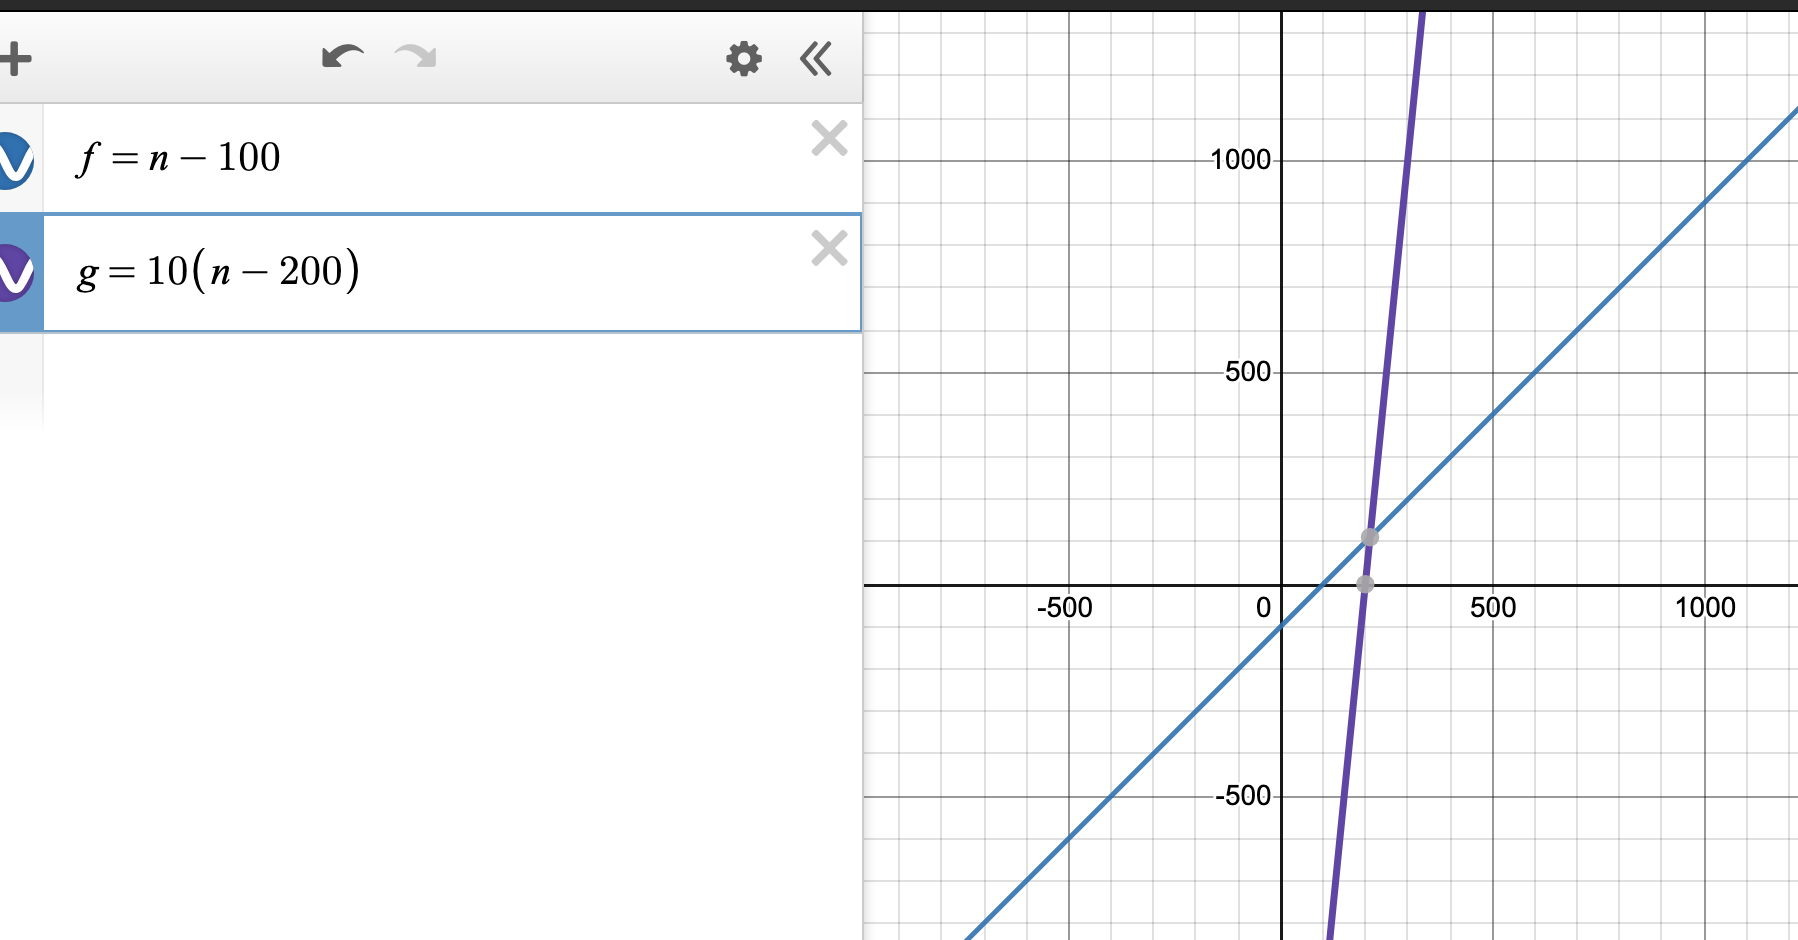
\includegraphics[width=0.9\linewidth, height=4cm]{a)big O.png}     
    \caption{Big O}
    \end{subfigure}
    \begin{subfigure}{0.5\textwidth}
    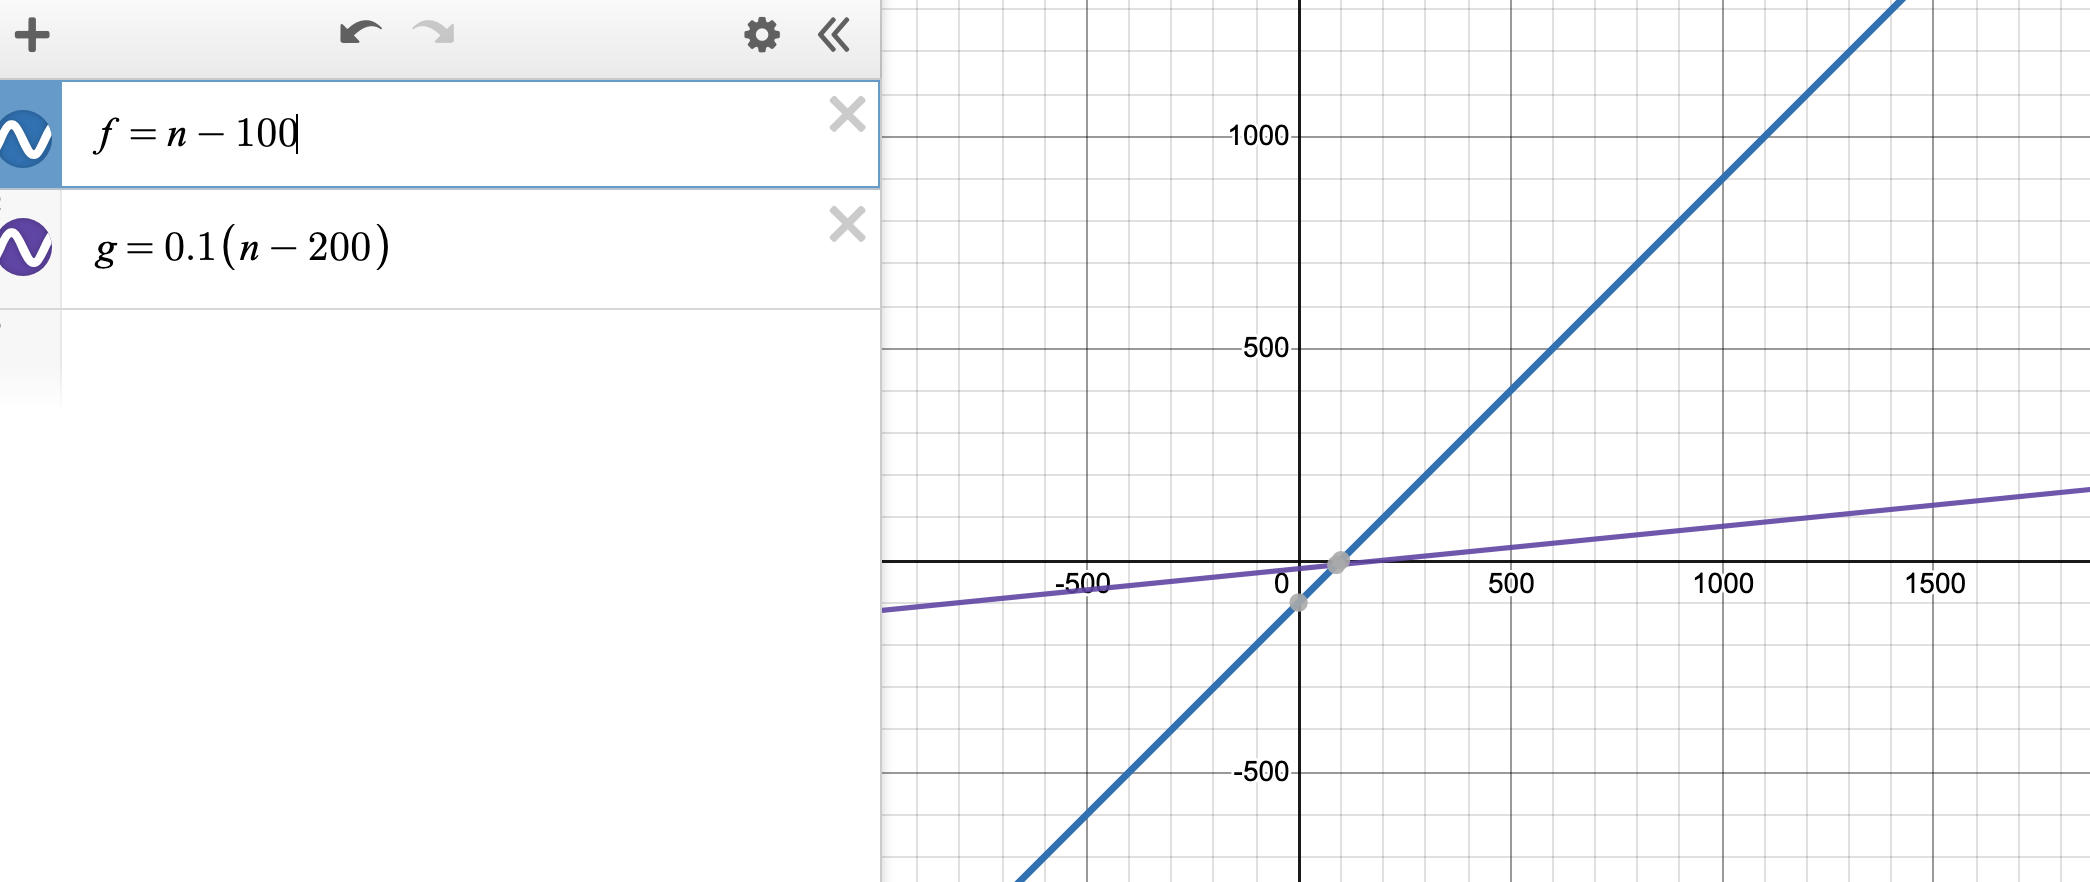
\includegraphics[width=0.9\linewidth, height=4cm]{a) big omega.png}
    \caption{Big Omega}
    \label{fig:subim2}
    \end{subfigure}
    \caption{Image for a)}
    \label{fig:image2}
\end{figure}

\begin{figure}[h]
\item 
No matter how small C is C*g(n) can always bigger than f(n) when n$\ge$n0, so there's f = O(g)  %% this is b
    
    \begin{subfigure}{0.5\textwidth}
    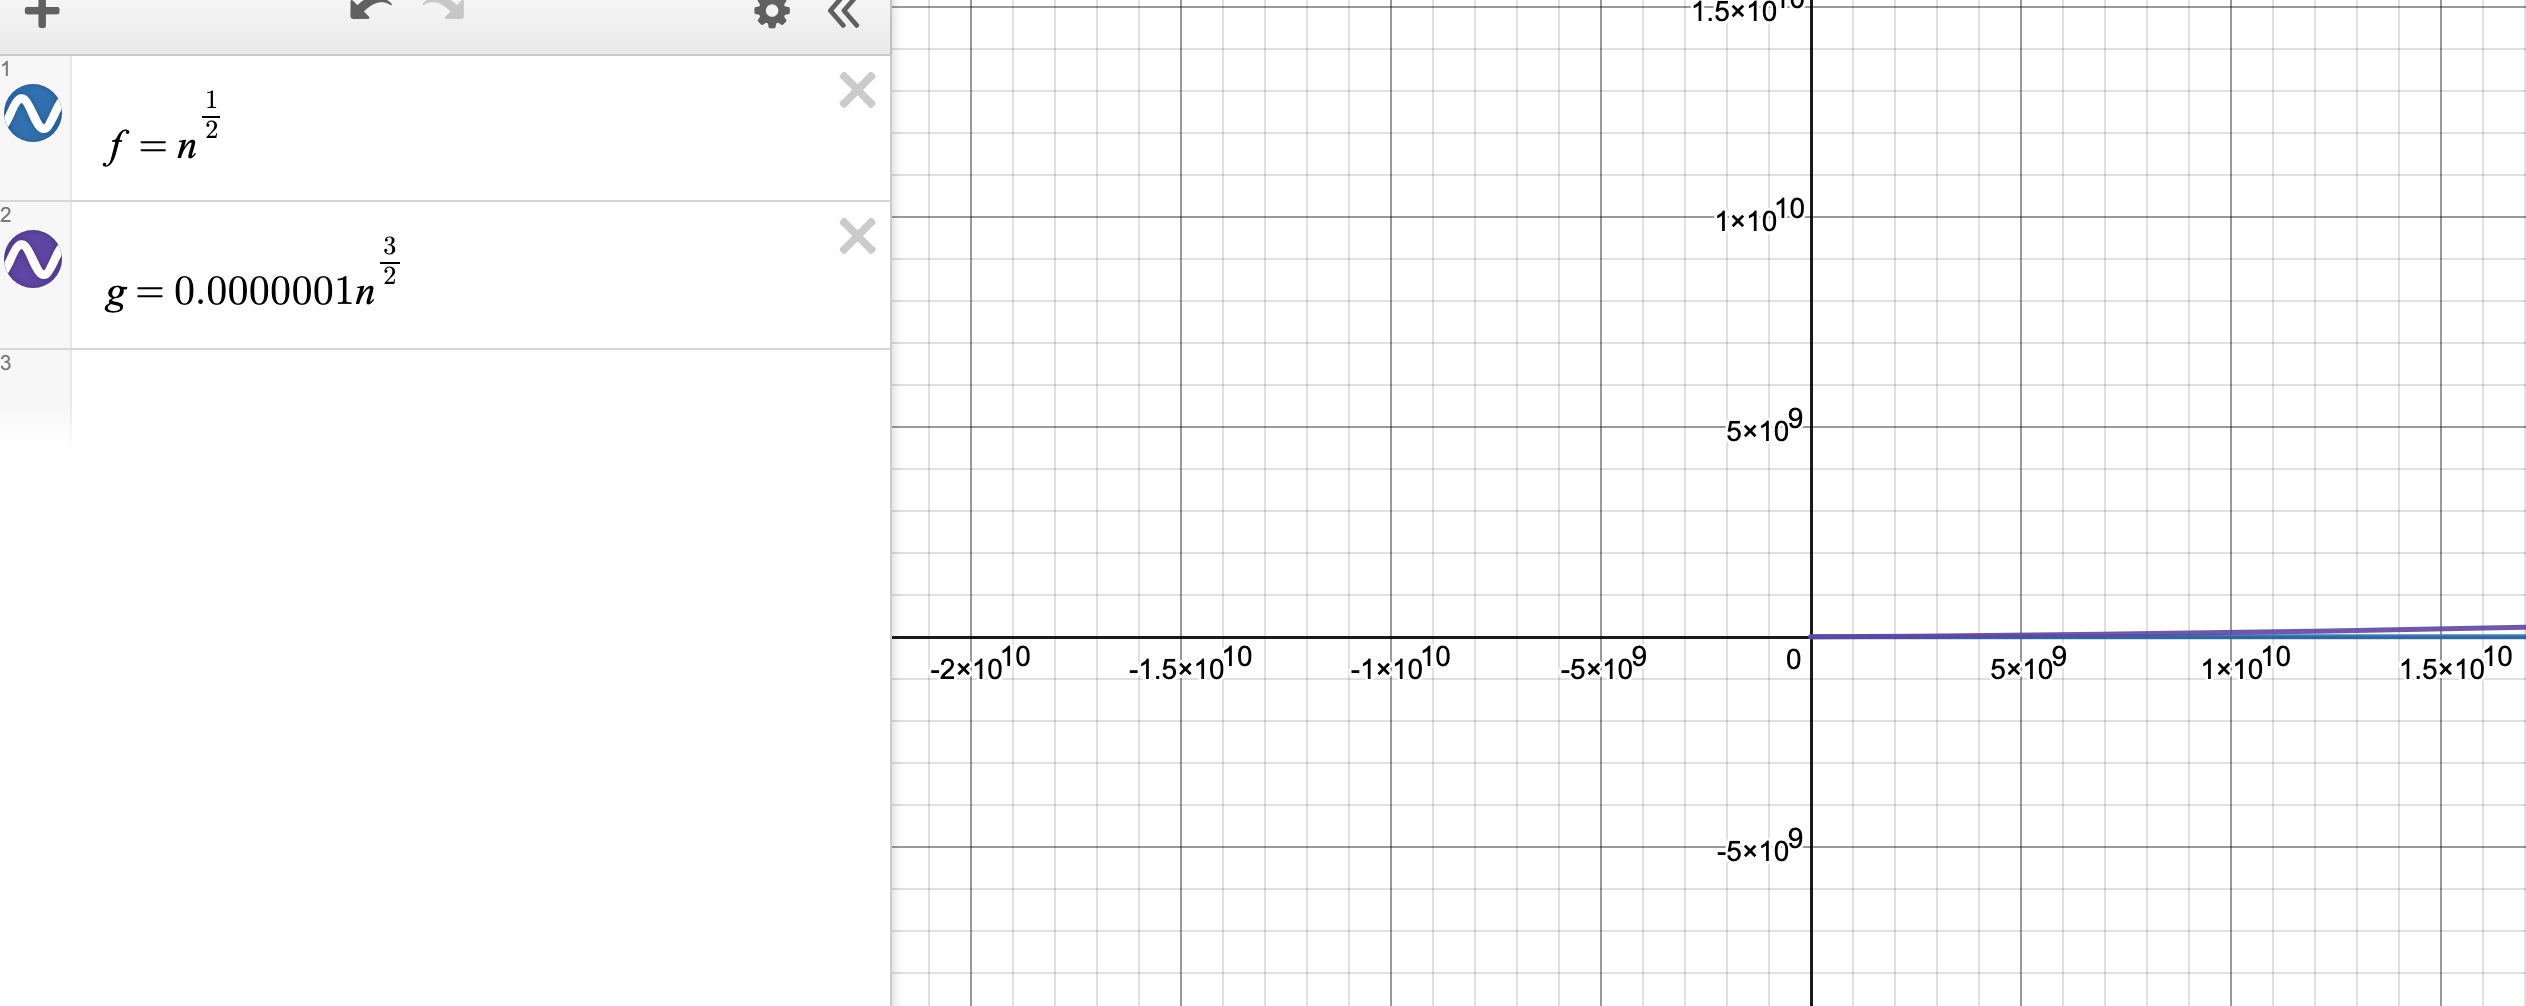
\includegraphics[width=0.9\linewidth, height=4cm]{b)big o.png }
    \caption{Big O}
    \label{fig:subim1}
    \end{subfigure}
    \caption{Image for b)}
    \label{fig:image2}
\end{figure}
\begin{figure}[h]
\item %%this is c
There is C and C' make $C*g(n) \le f(n) \le C'*g(n)$, so  there's f = O(g), f = Omega (g) and f = Theta(g)\\
    \begin{subfigure}{0.5\textwidth}
    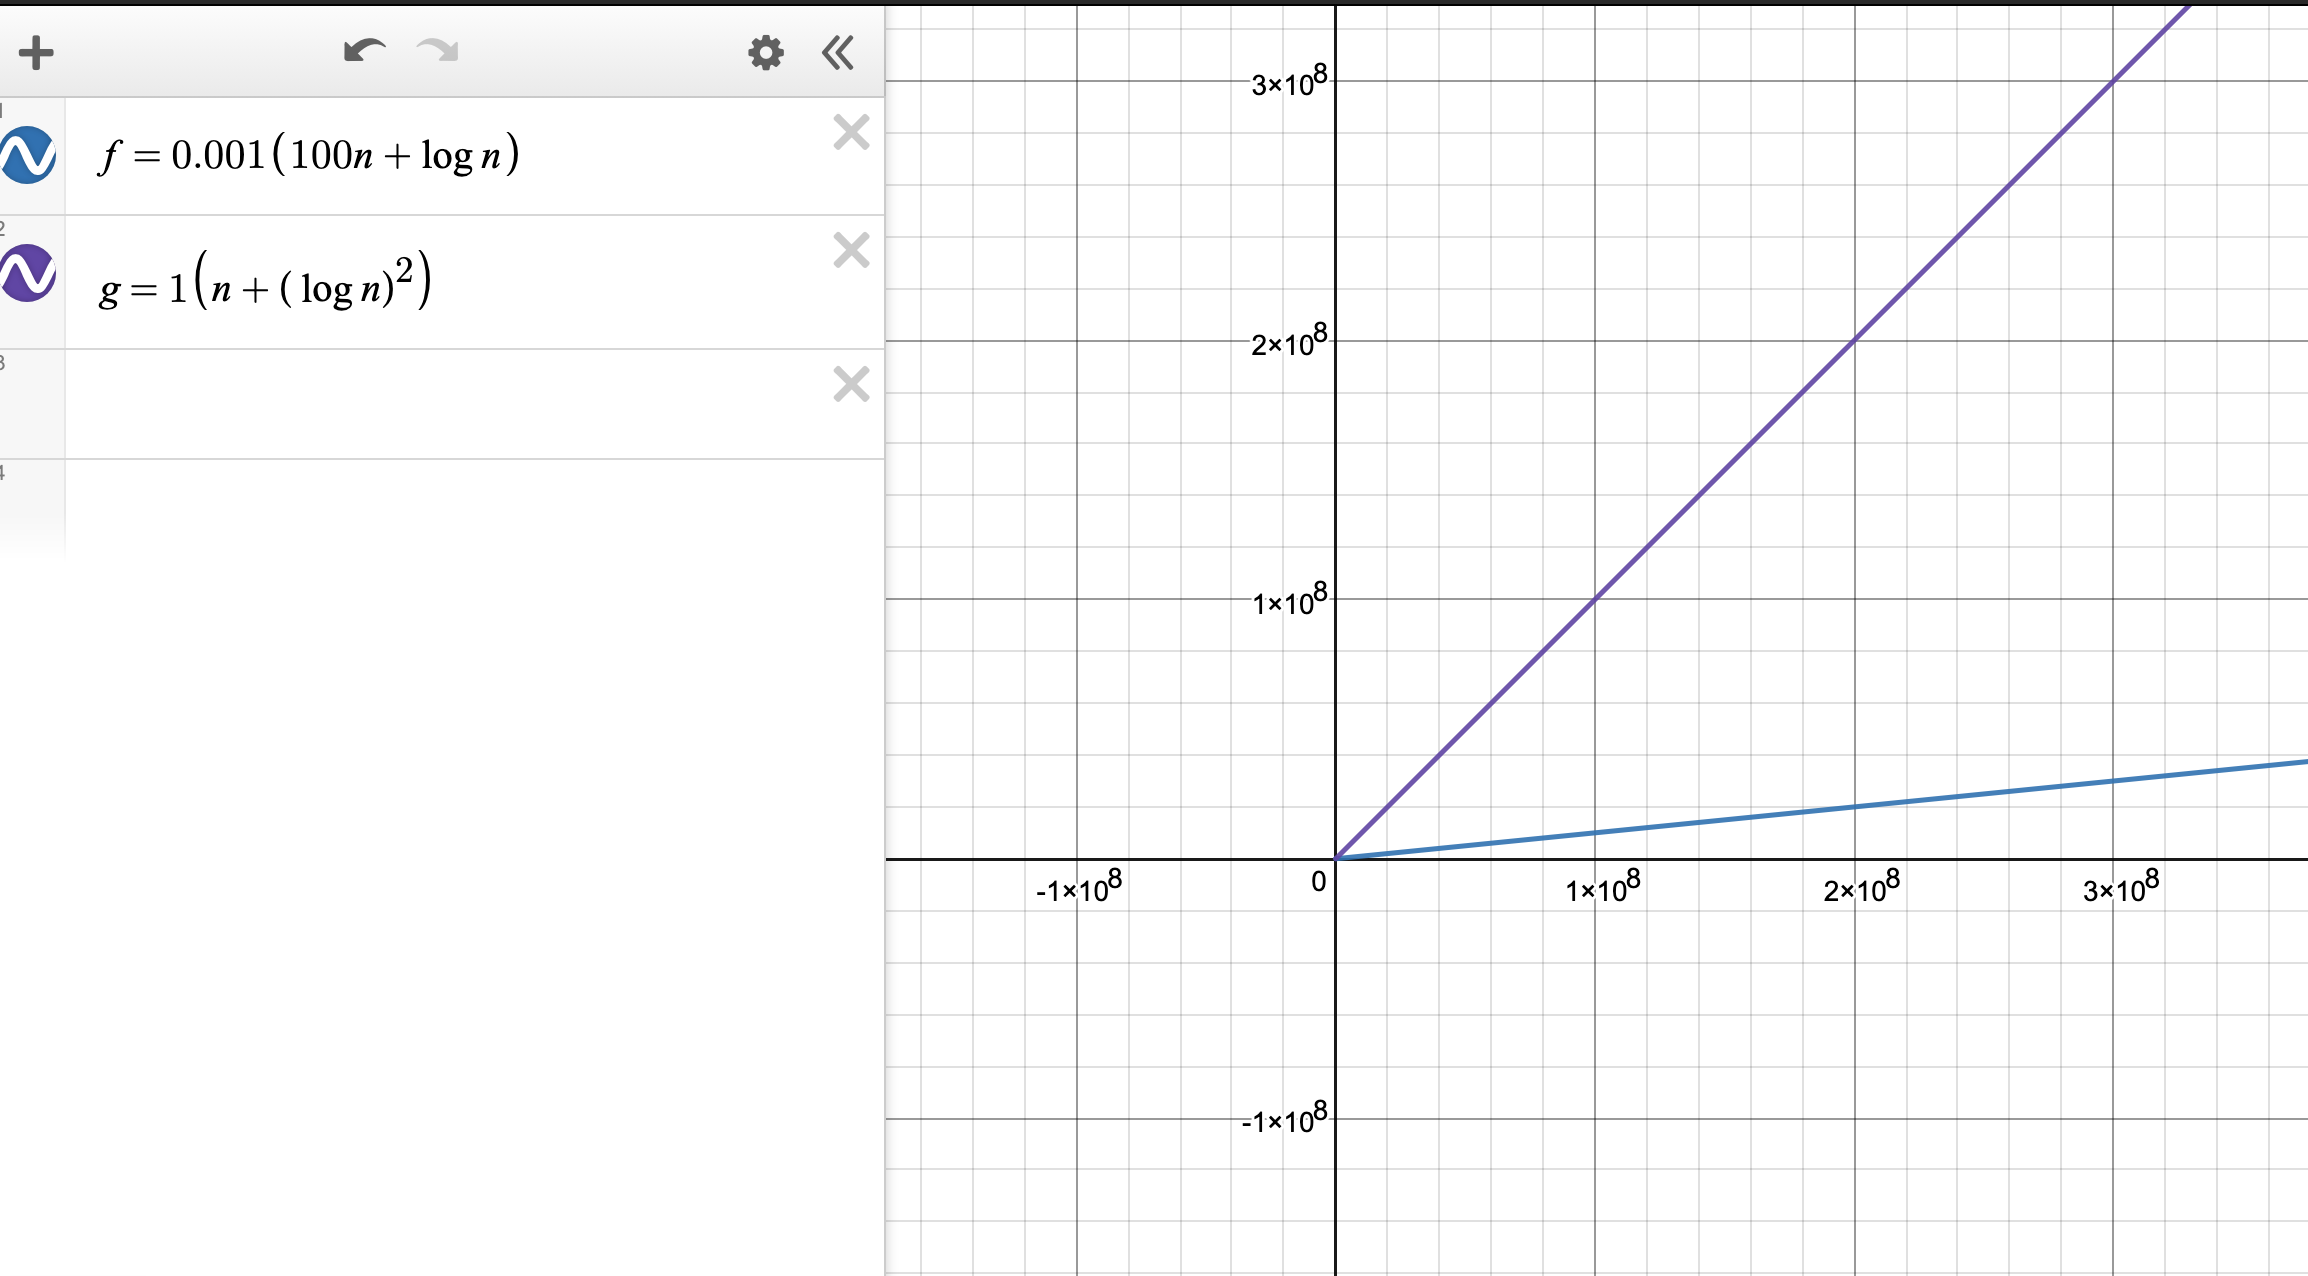
\includegraphics[width=0.9\linewidth, height=4cm]{c)big O.png}
    \caption{Big O}
    \label{fig:subim1}
    \end{subfigure}
    \begin{subfigure}{0.5\textwidth}
    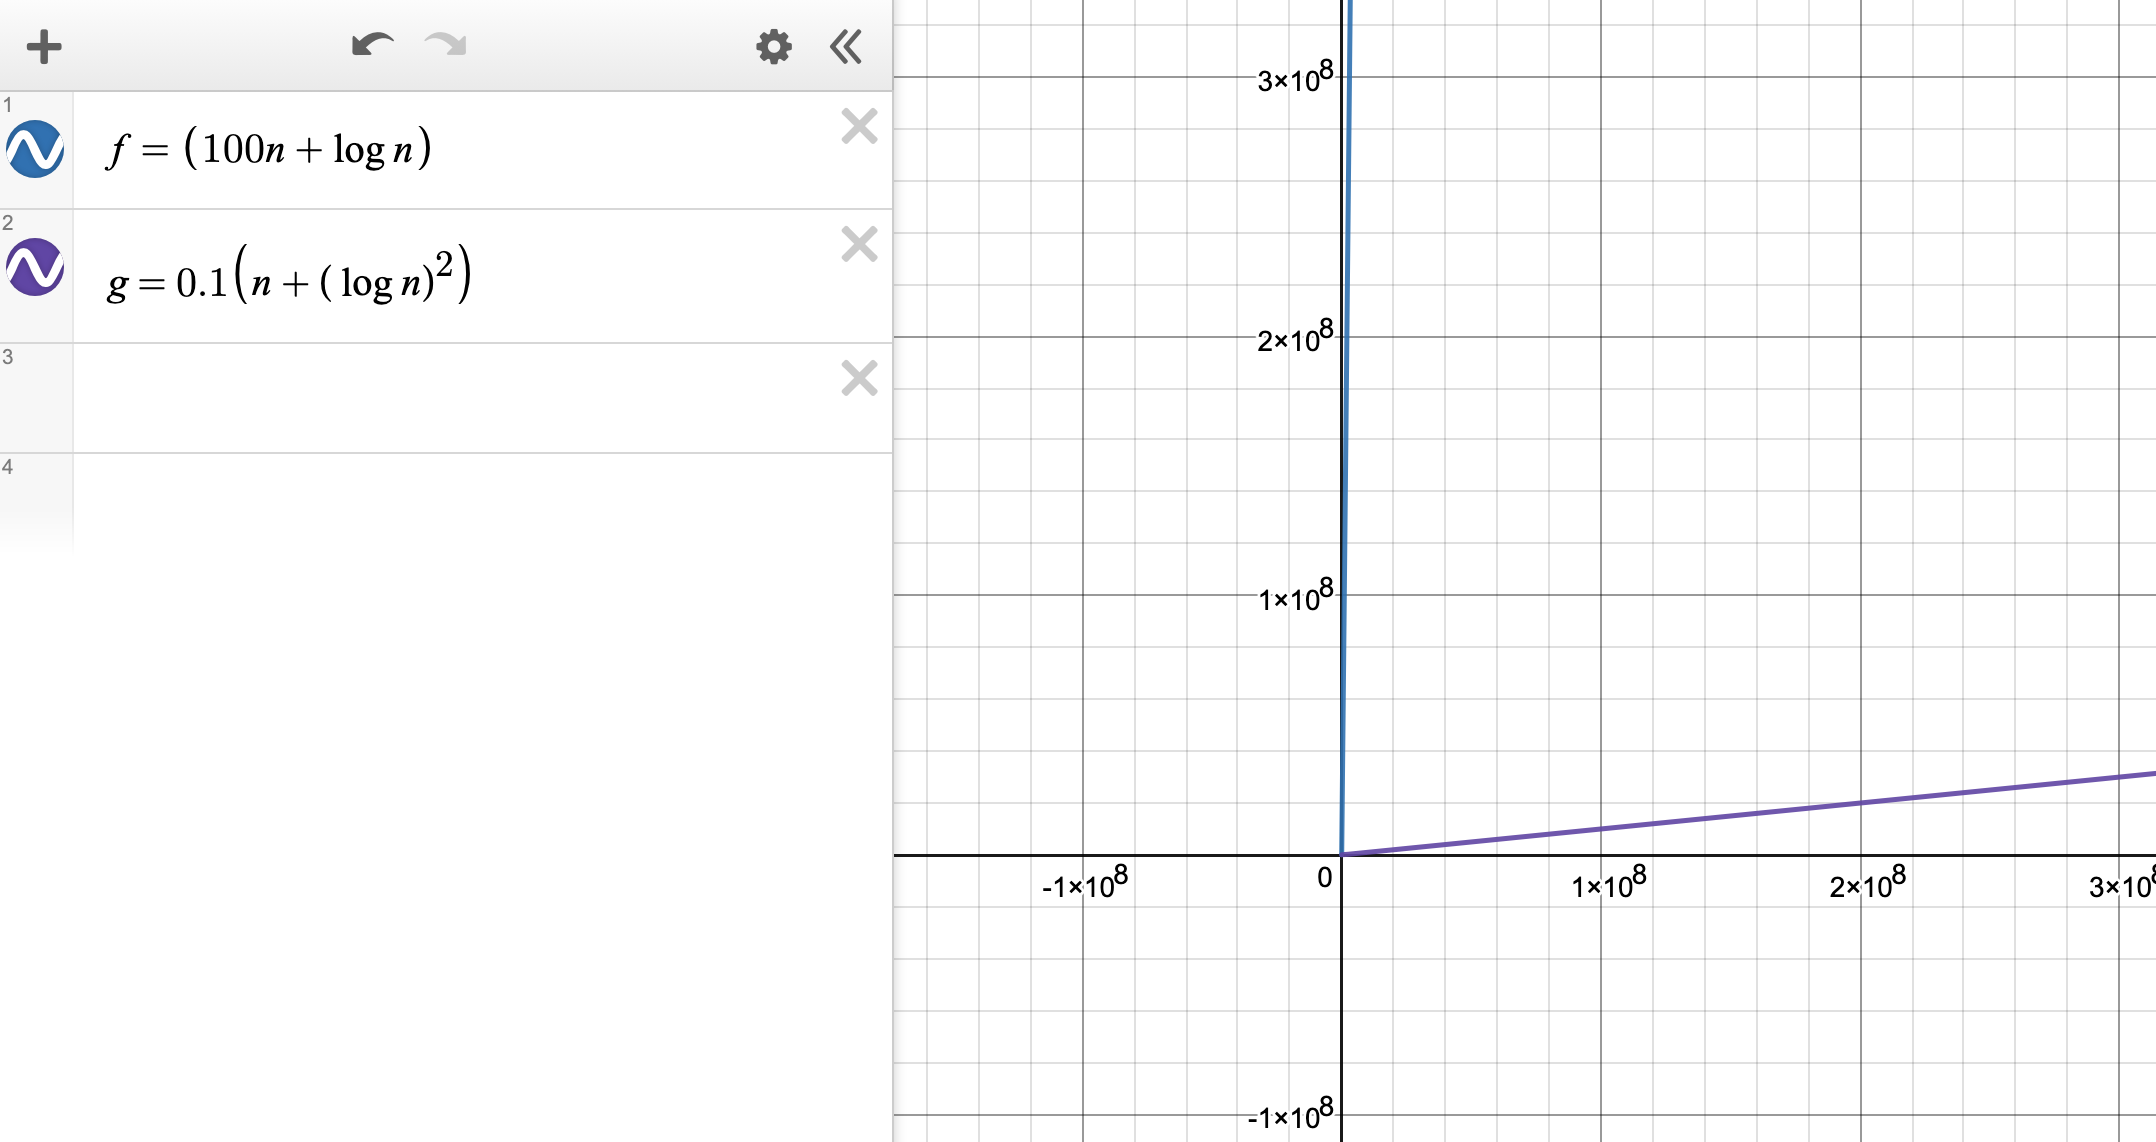
\includegraphics[width=0.9\linewidth, height=4cm]{c) big omega.png}
    \caption{Big Omega}
    \label{fig:subim2}
    \end{subfigure}
    \caption{Image for c)}
    \label{fig:image2}
\end{figure}
\item  %% this is d 

There is C and C' make $C*g(n) \le f(n) \le C'*g(n)$, so  there's f = O(g), f = Omega (g) and f = Theta(g)\\
    \begin{figure}[h]
    \begin{subfigure}{0.5\textwidth}
    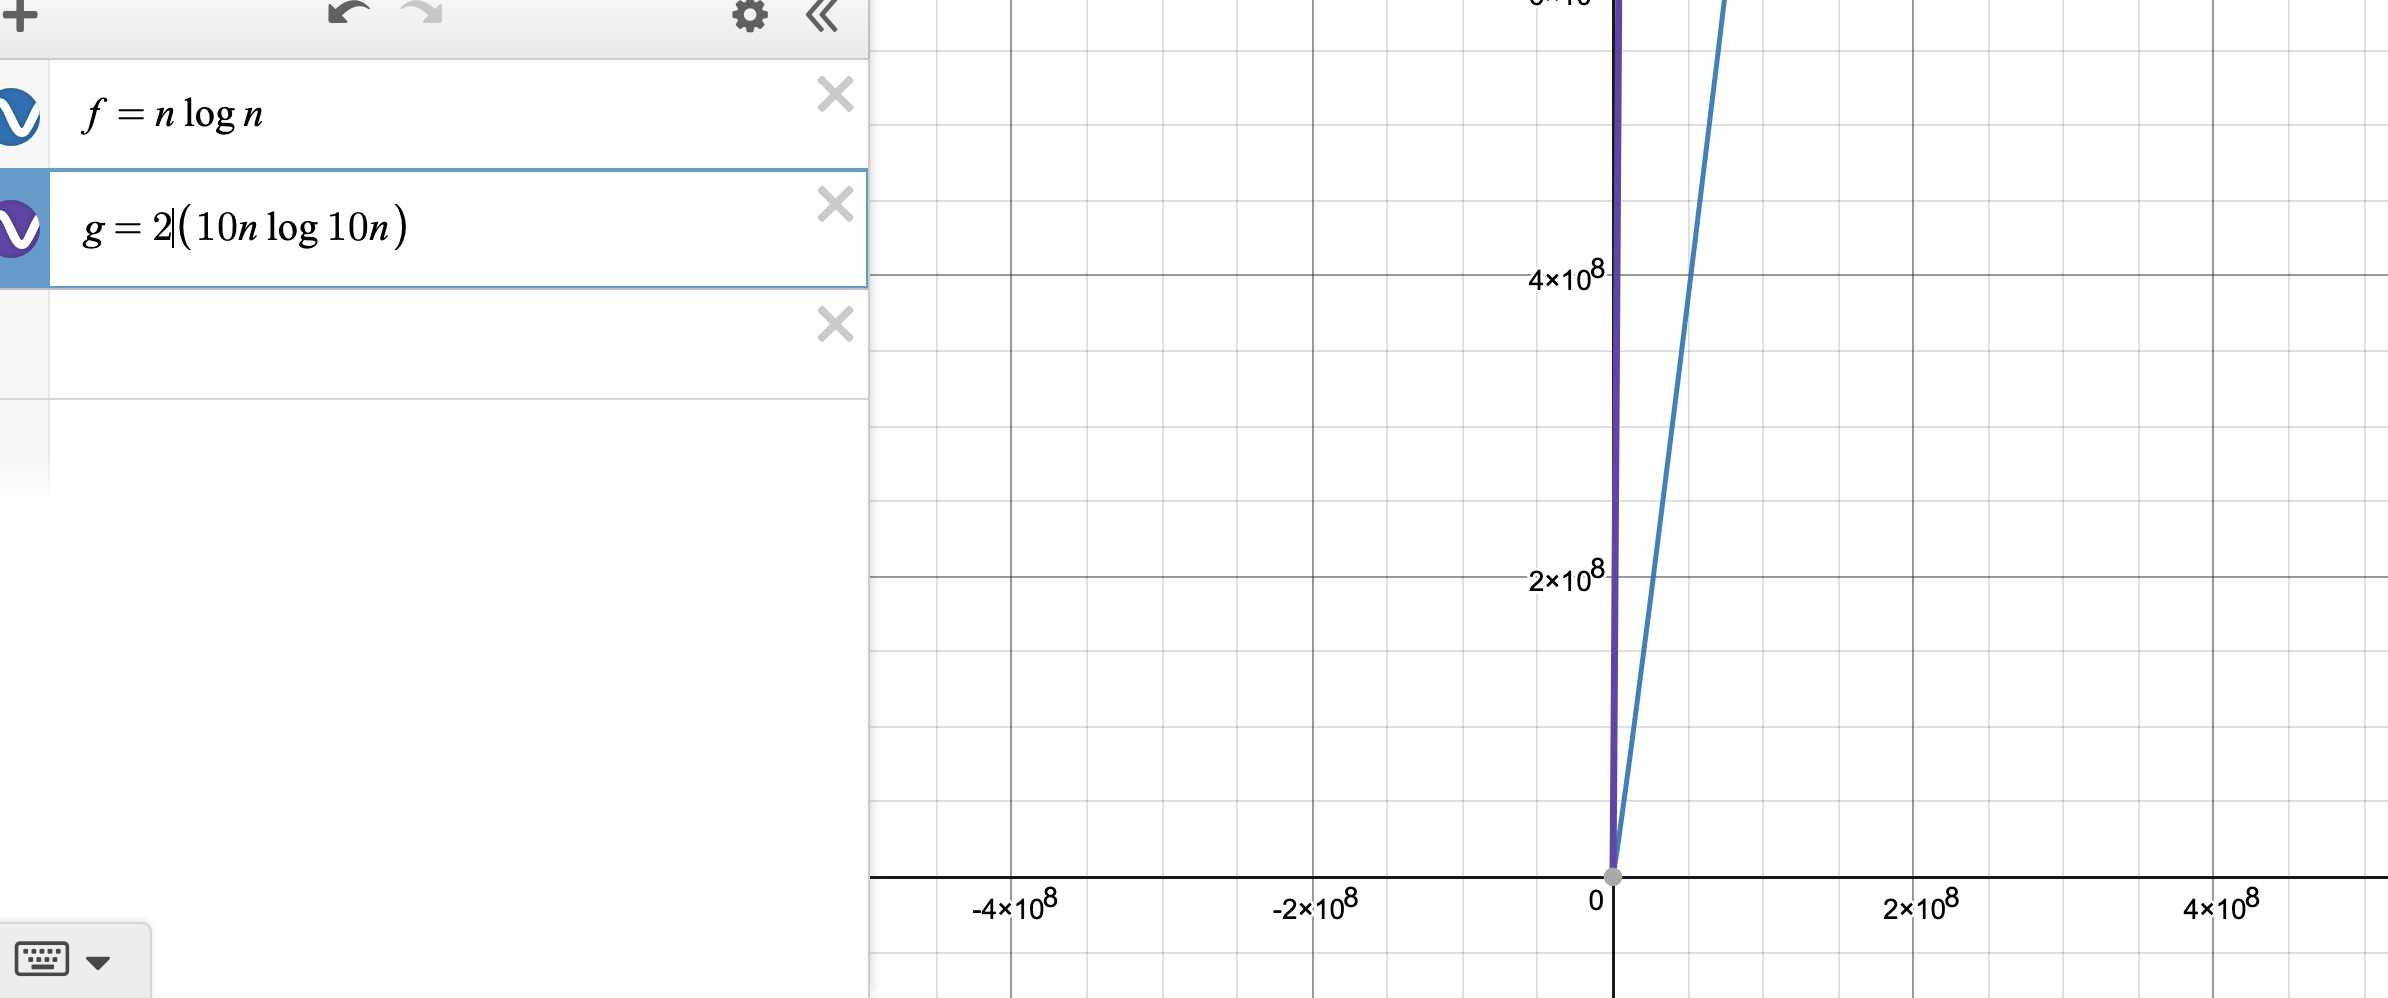
\includegraphics[width=0.9\linewidth, height=4cm]{d) big O.png}
    \caption{Big O}
    \label{fig:subim1}
    \end{subfigure}
    \begin{subfigure}{0.5\textwidth}
    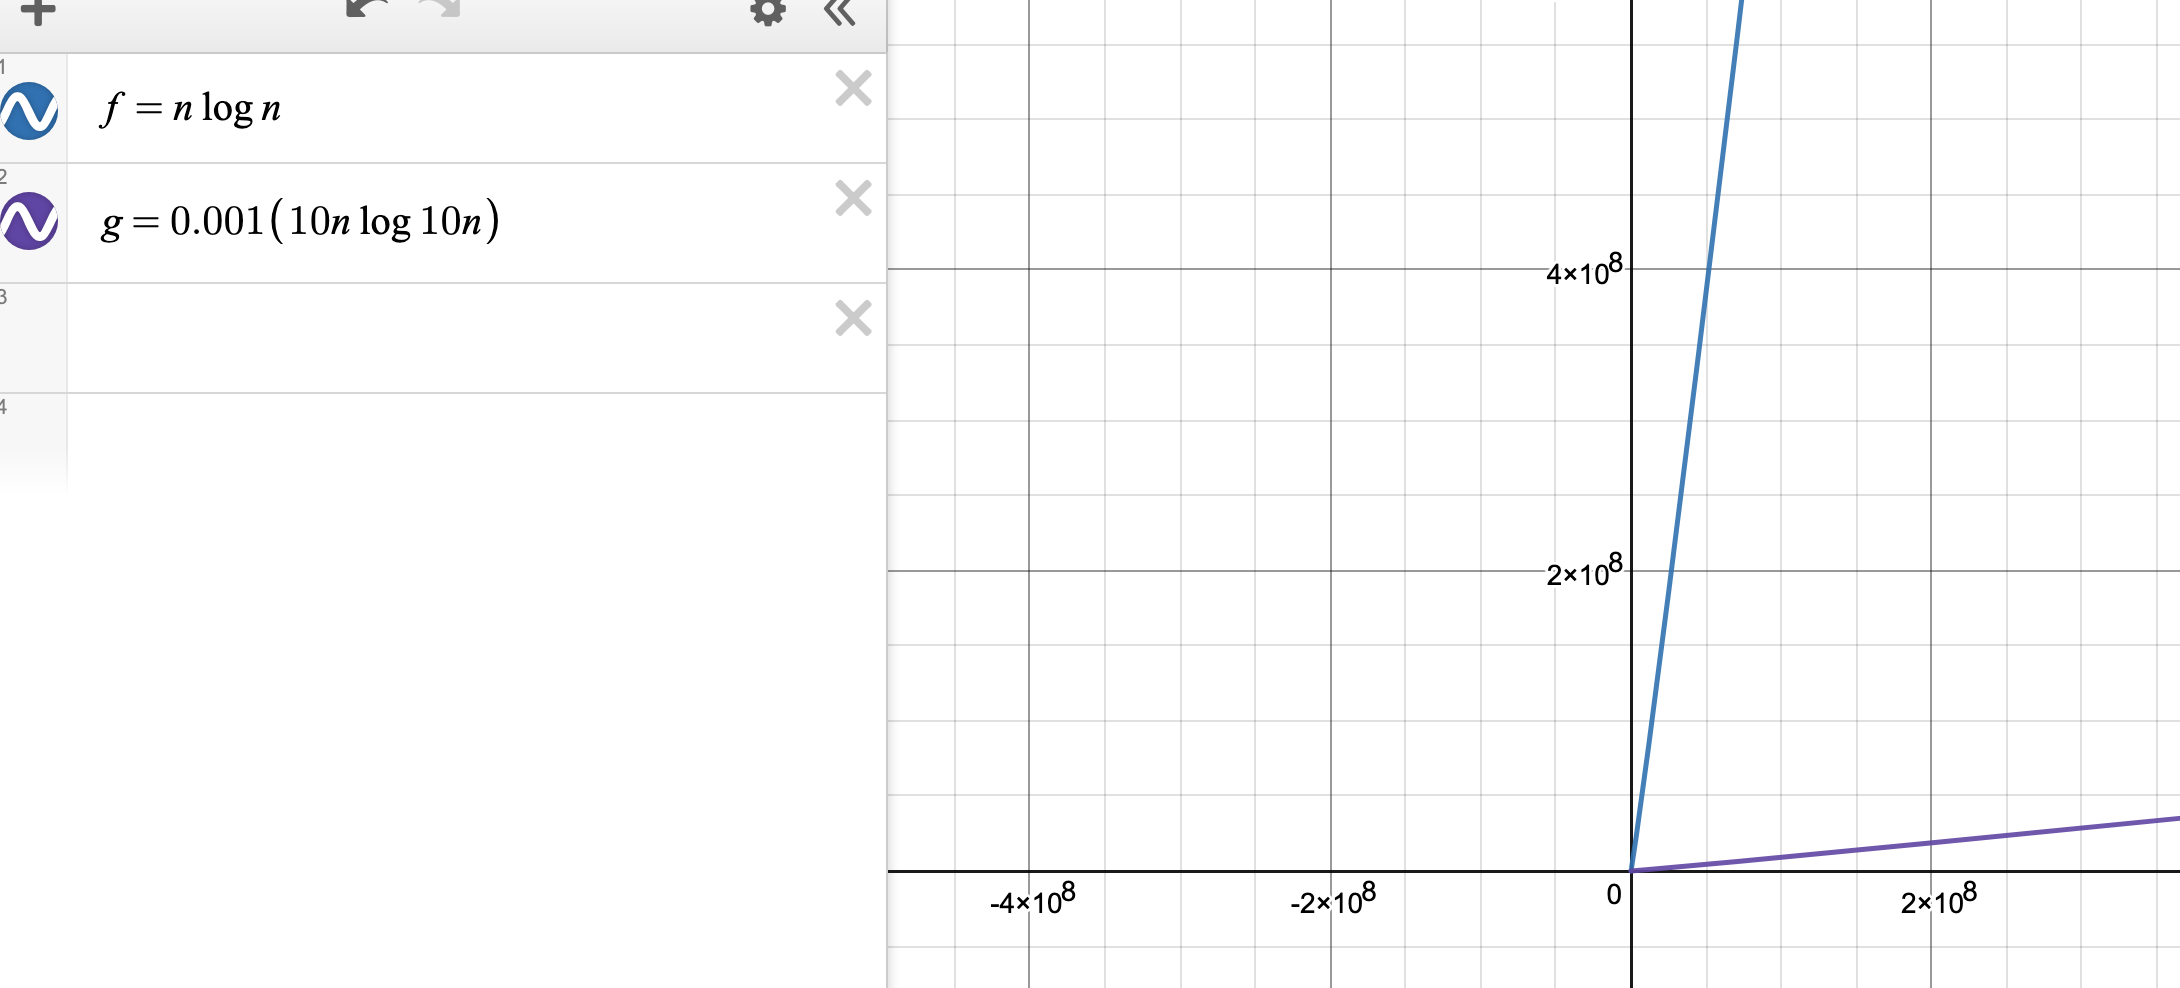
\includegraphics[width=0.9\linewidth, height=4cm]{d) big omega .png}
    \caption{Big Omega}
    \label{fig:subim2}
    \end{subfigure}
    \caption{Image for d)}
    \label{fig:image2}
    \end{figure}

\begin{figure}[h]
\item %% this is e
There is C and C' make $C*g(n) \le f(n) \le C'*g(n)$, so  there's f = O(g), f = Omega (g) and f = Theta(g)\\
    \begin{subfigure}{0.5\textwidth}
    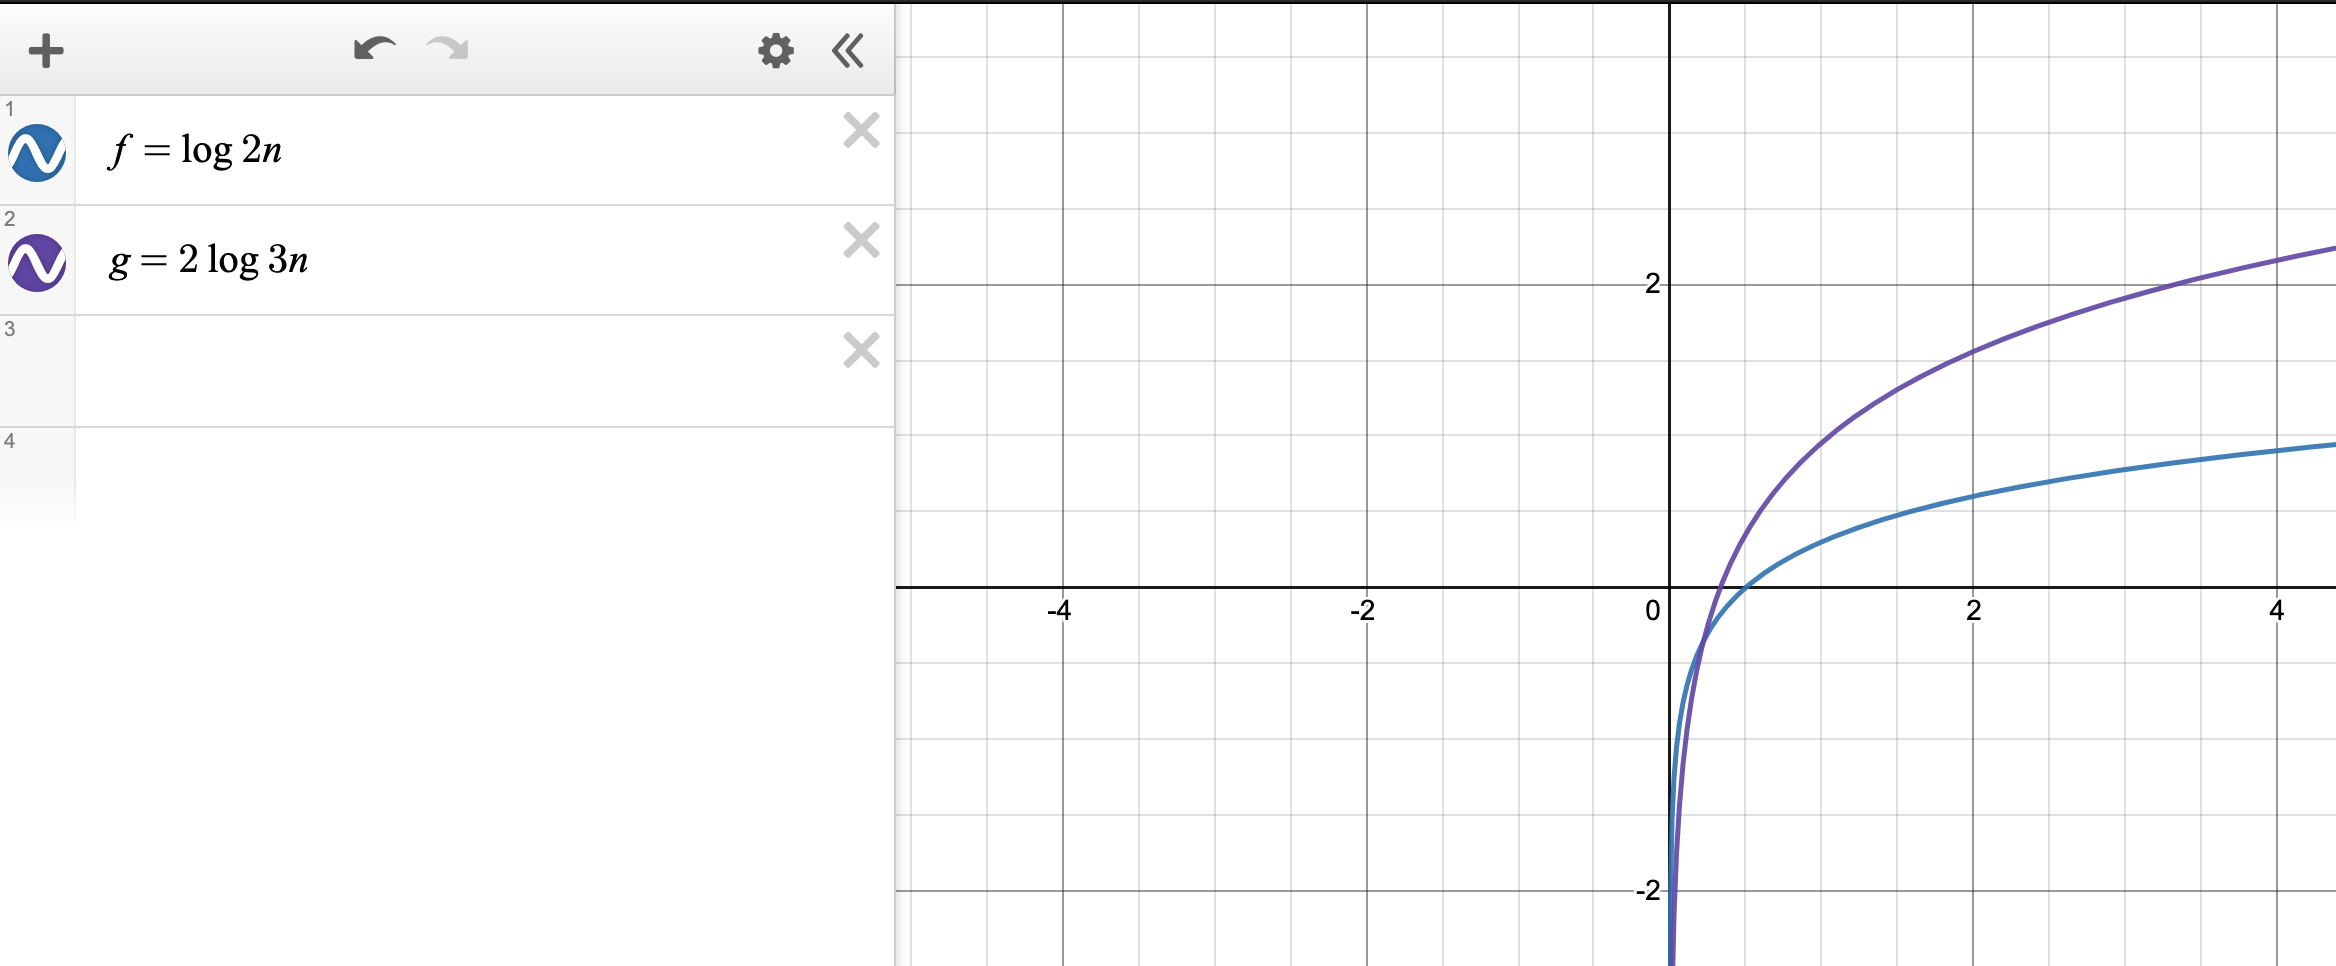
\includegraphics[width=0.9\linewidth, height=4cm]{e) big O.png}
    \caption{Big O}
    \label{fig:subim1}
    \end{subfigure}
    \begin{subfigure}{0.5\textwidth}
    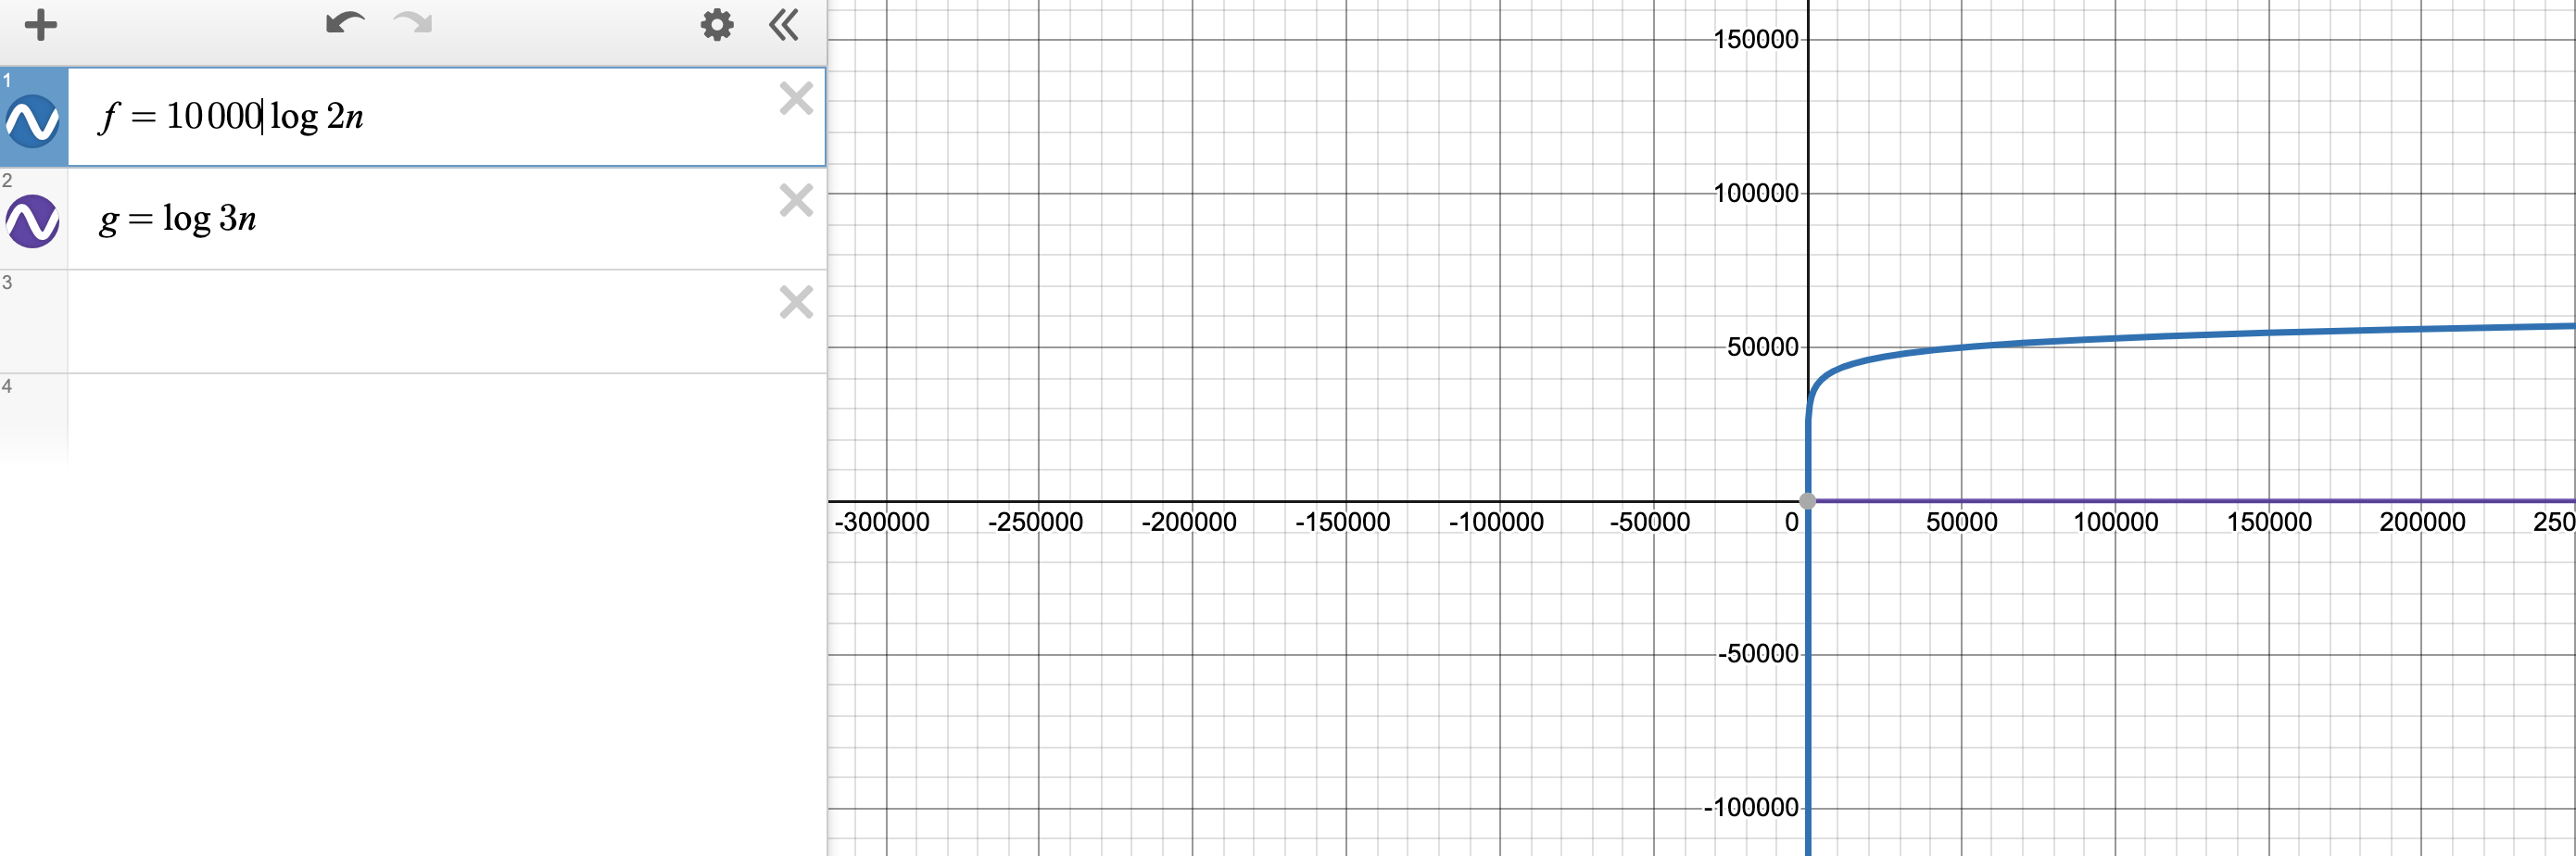
\includegraphics[width=0.9\linewidth, height=4cm]{ e) big omega.png}
    \caption{Big Omega}
    \label{fig:subim2}
    \end{subfigure}
    \caption{Image for e)}
    \label{fig:image2}
\end{figure}

\begin{figure}[h]
\item %% this is f
There is C and C' make $C*g(n) \le f(n) \le C'*g(n)$, so  there's f = O(g), f = Omega (g) and f = Theta(g)\\
    
    \begin{subfigure}{0.5\textwidth}
    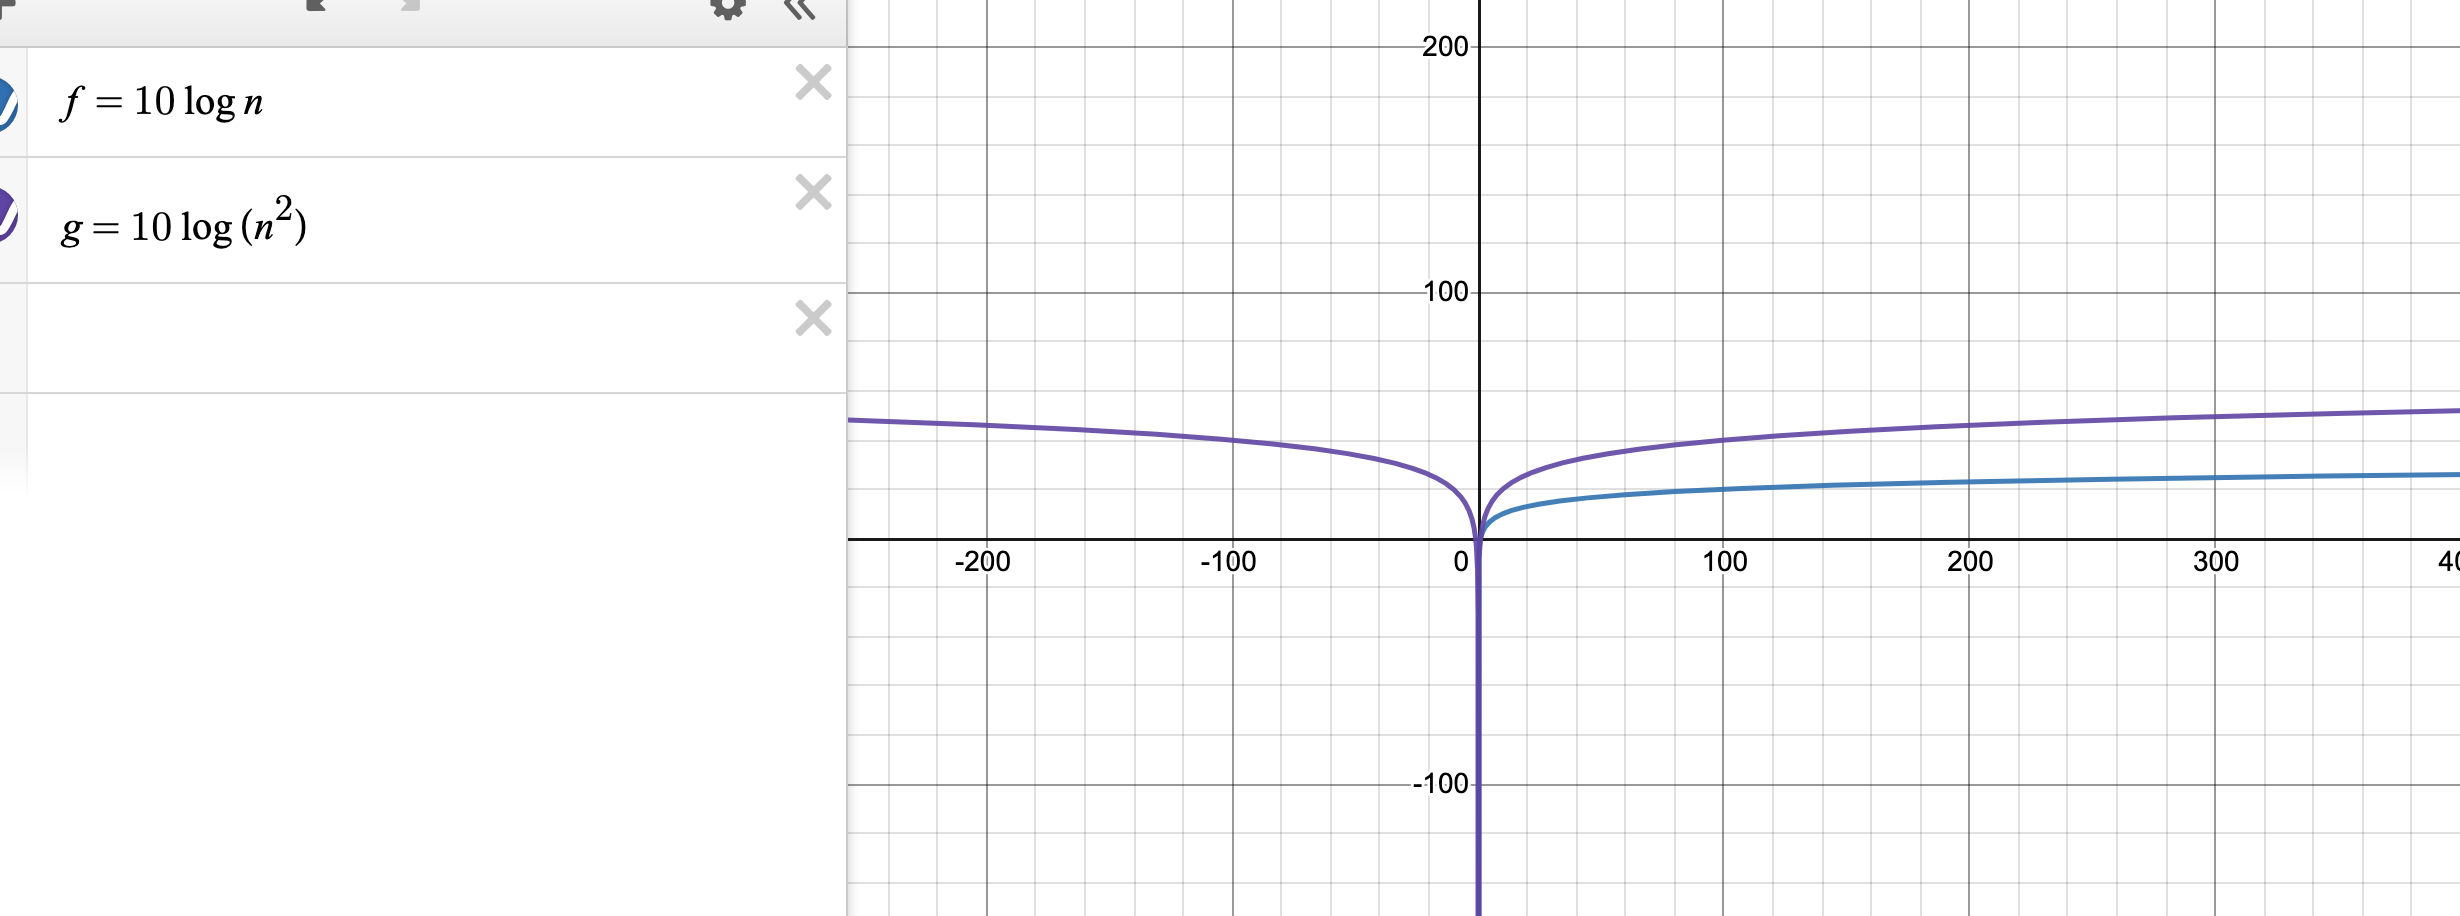
\includegraphics[width=0.9\linewidth, height=4cm]{f) big O.png}
    \caption{Big O}
    \label{fig:subim1}
    \end{subfigure}
    \begin{subfigure}{0.5\textwidth}
    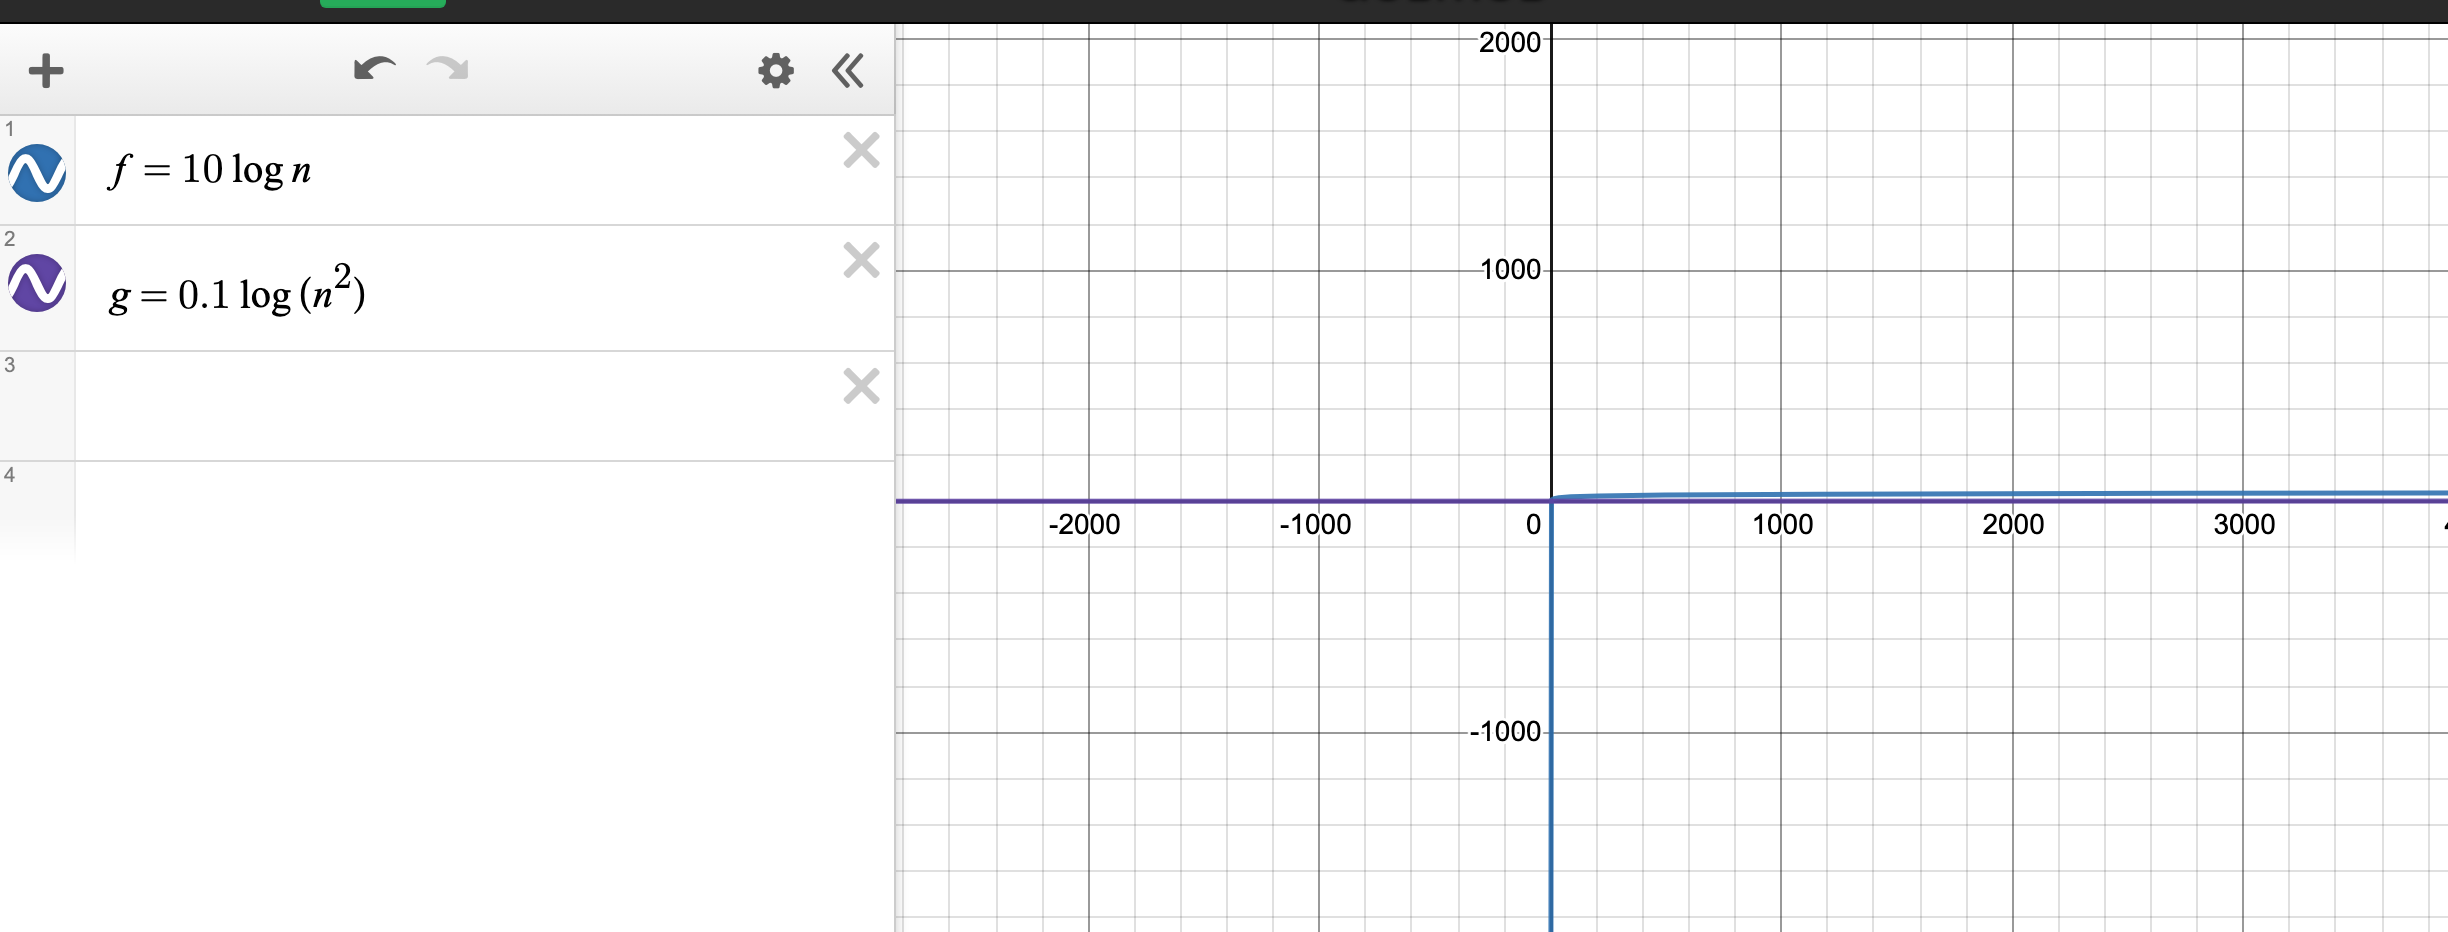
\includegraphics[width=0.9\linewidth, height=4cm]{f) big omega.png}
    \caption{Big Omega}
    \label{fig:subim2}
    \end{subfigure}
    \caption{Image for f)}
    \label{fig:image2}
\end{figure}

\begin{figure}[h]
\item %% this is g
There is C and C' make $C*g(n) \le f(n) \le C'*g(n)$, so  there's f = O(g), f = Omega (g) and f = Theta(g)\\
    \begin{subfigure}{0.5\textwidth}
    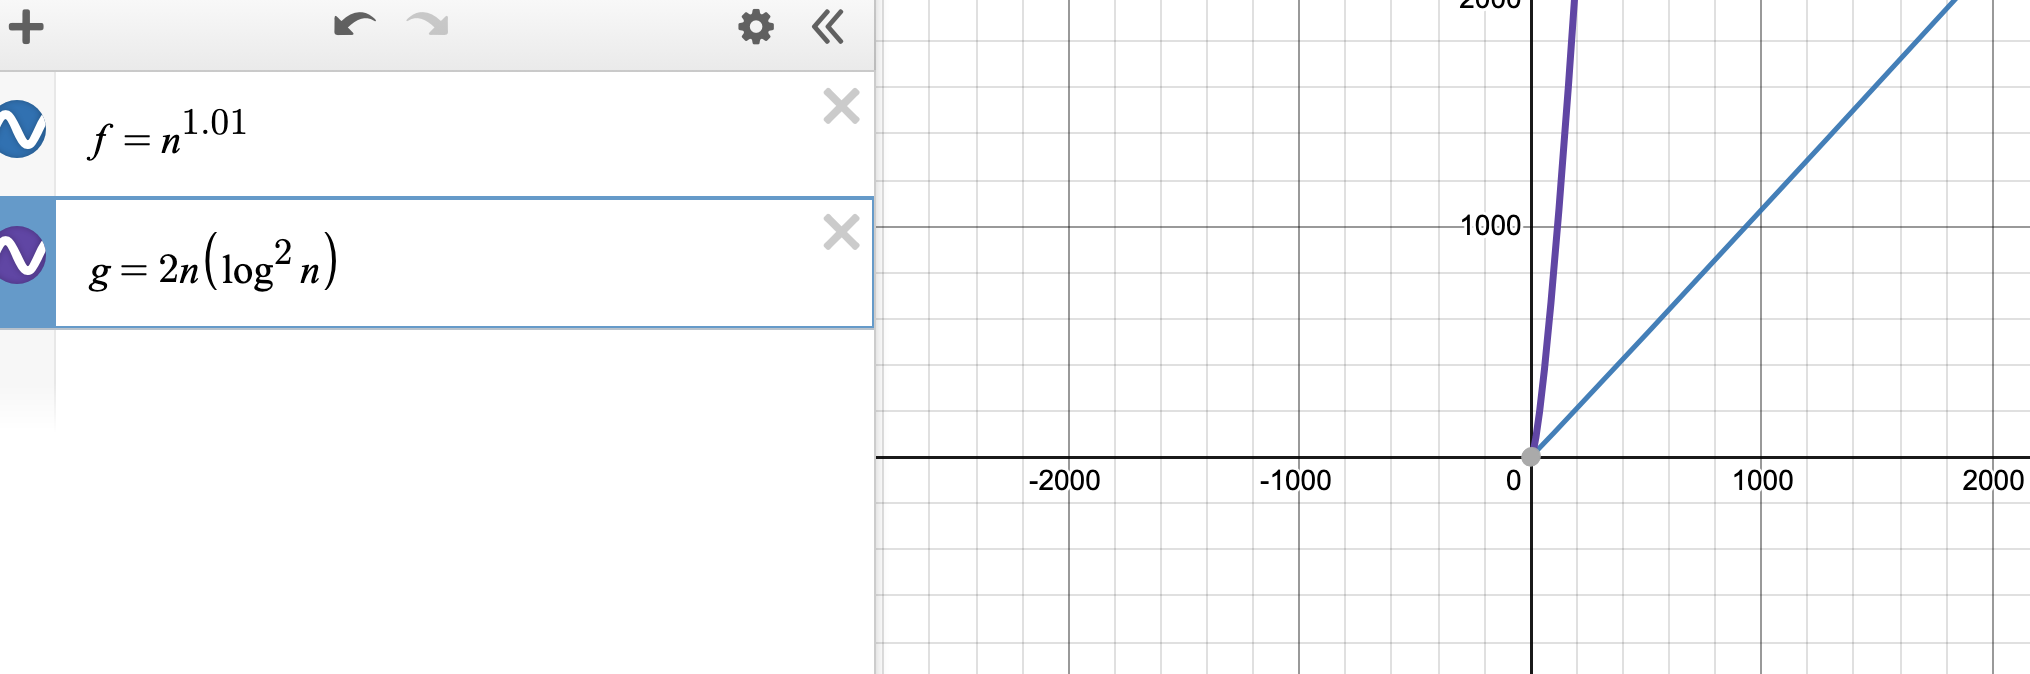
\includegraphics[width=0.9\linewidth, height=4cm]{g) big O.png}
    \caption{Big O}
    \label{fig:subim1}
    \end{subfigure}
    \begin{subfigure}{0.5\textwidth}
    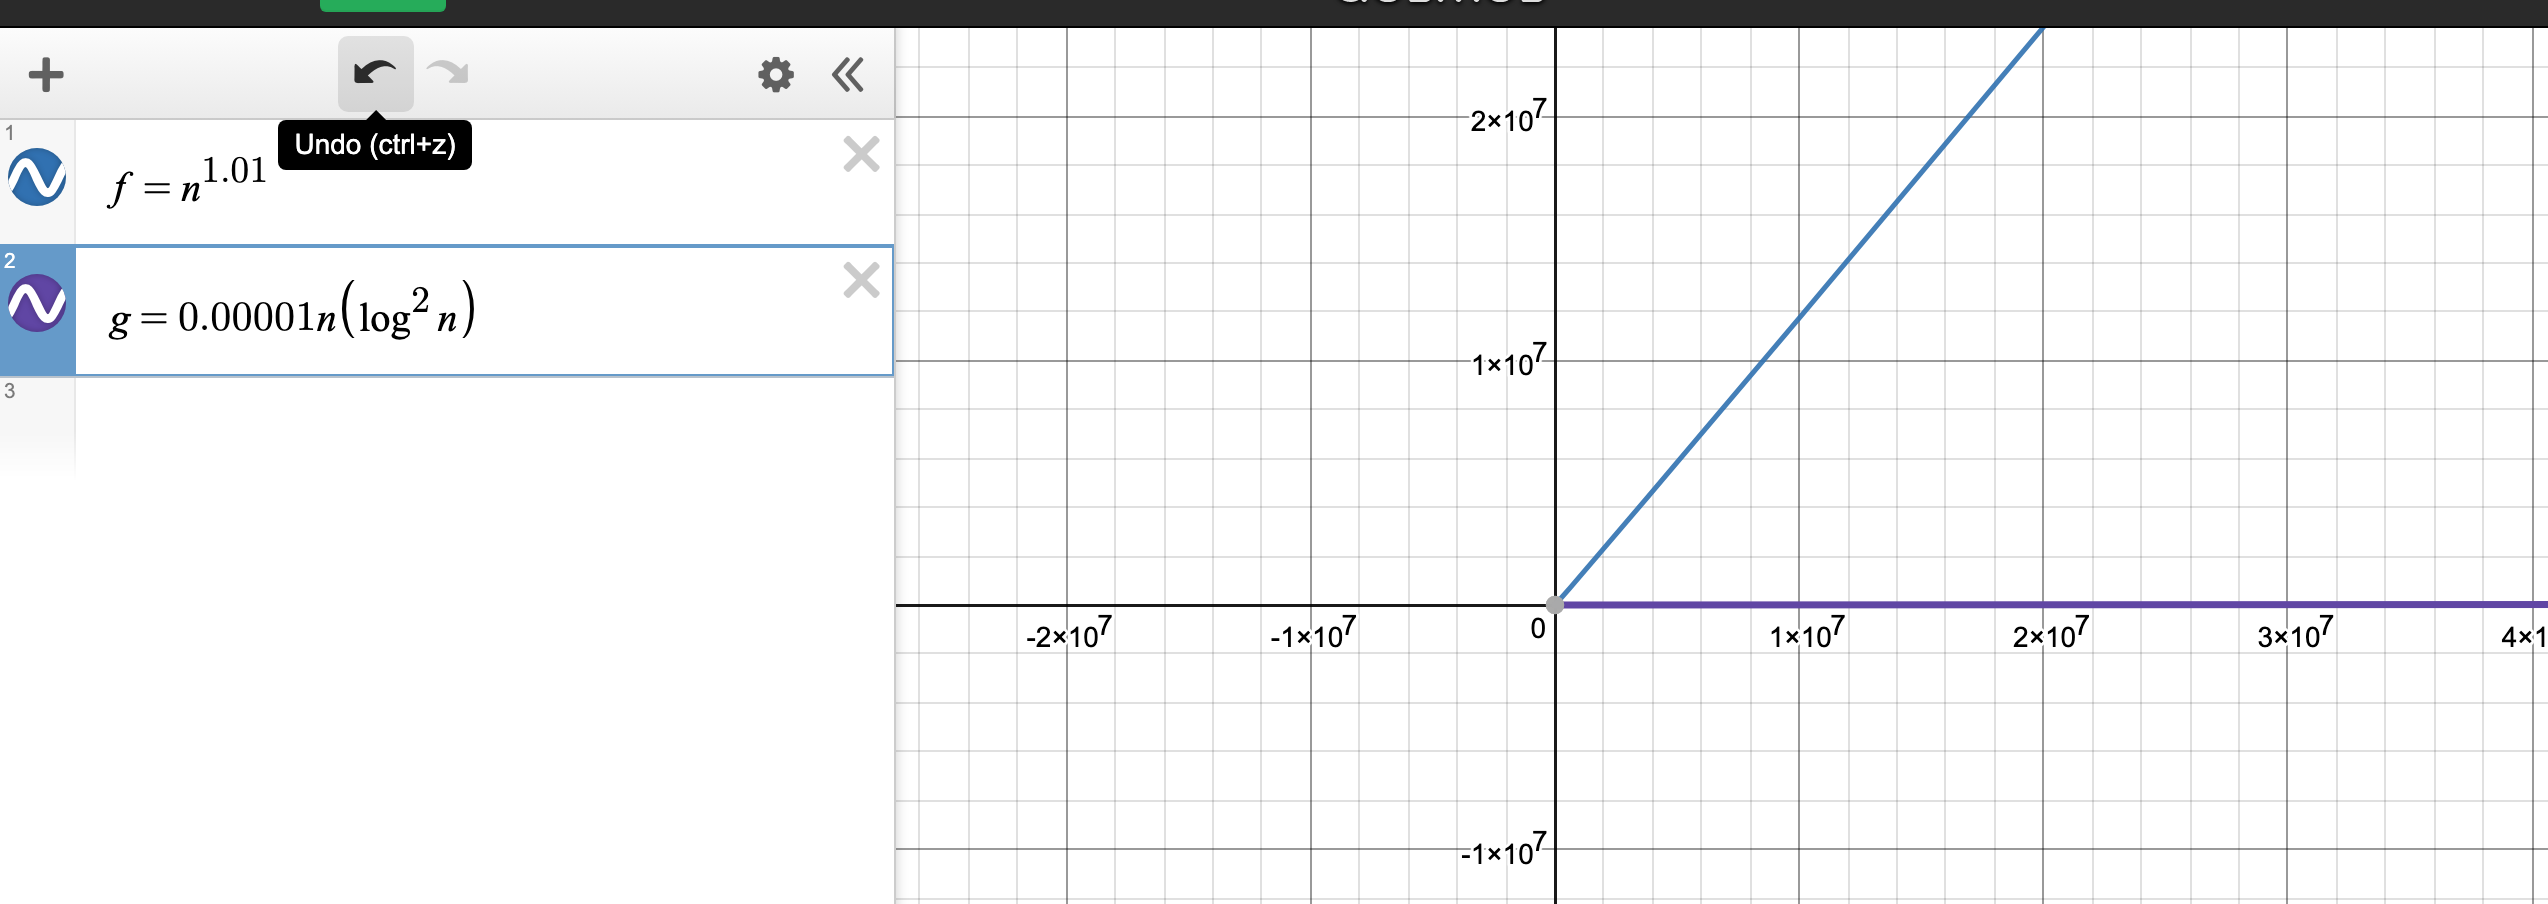
\includegraphics[width=0.9\linewidth, height=4cm]{g) big omega.png}
    \caption{Big Omega}
    \label{fig:subim2}
    \end{subfigure}
    \caption{Image for g)}
    \label{fig:image2}
    \end{figure}
    
\begin{figure}[h]
\item %% this is h
No matter how big C is, C*g(n) can always smaller than f(n) at some point when n $\ge $n0, so there's $f = \Omega(g)$\\
    \begin{subfigure}{0.5\textwidth}
    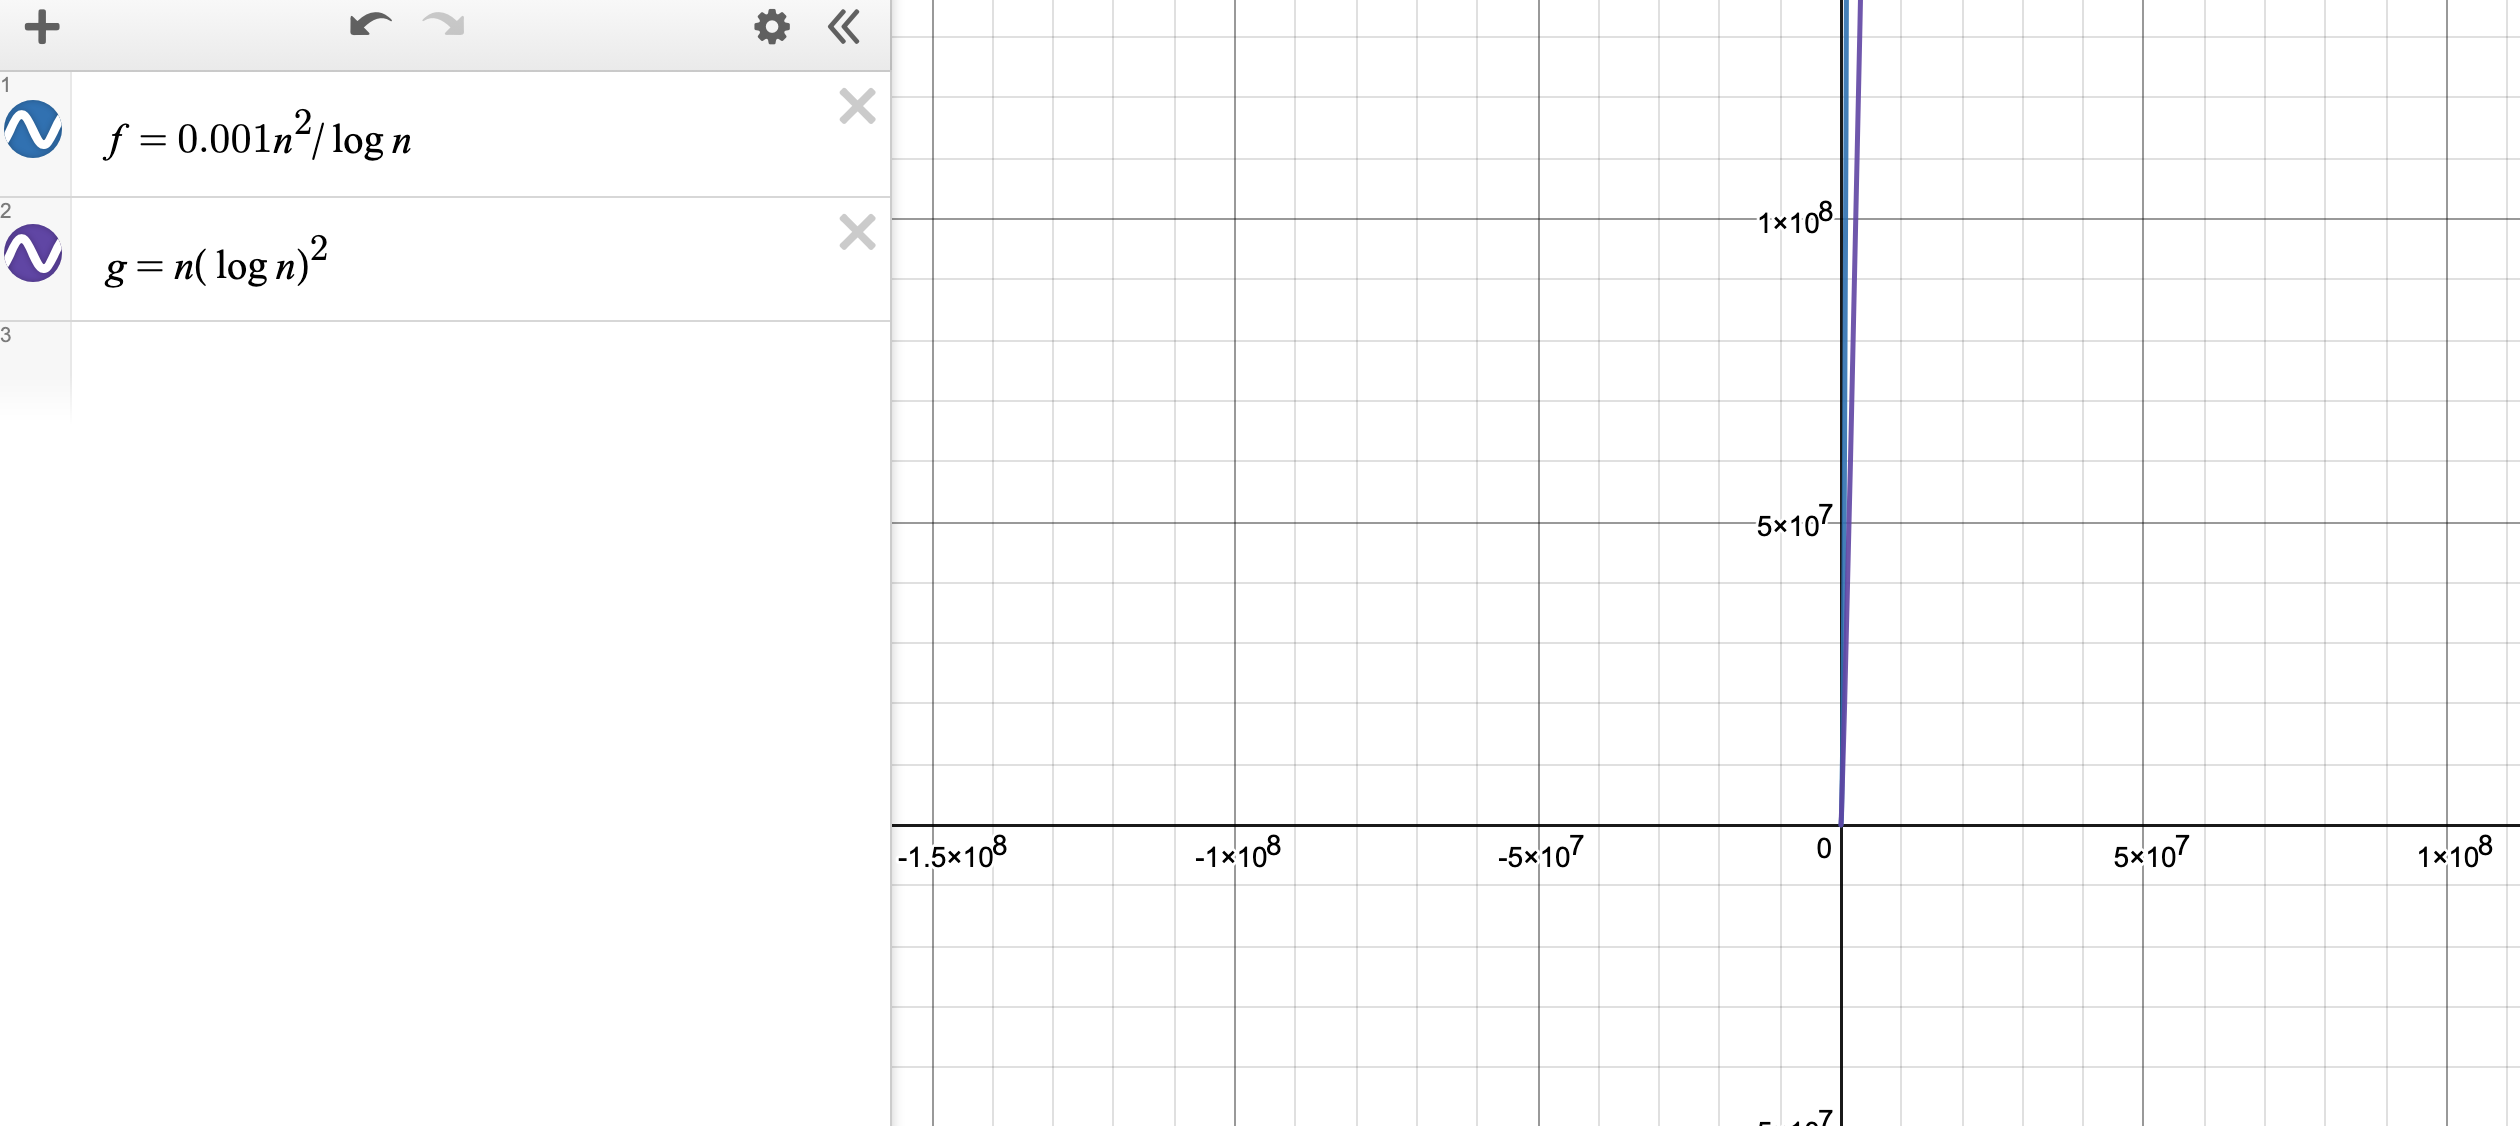
\includegraphics[width=0.9\linewidth, height=4cm]{h.big omega.png}
    \caption{Big omega}
    \label{fig:subim1}
    \end{subfigure}
    \caption{Image for h)}
    \label{fig:image2}
    \end{figure}
    
\begin{figure}[h]    
\item %% this is i
No matter how big C is, C*g(n) can always smaller than f(n) at some point when n $\ge $n0, so there's $f = \Omega(g)$\\
    \begin{subfigure}{0.5\textwidth}
    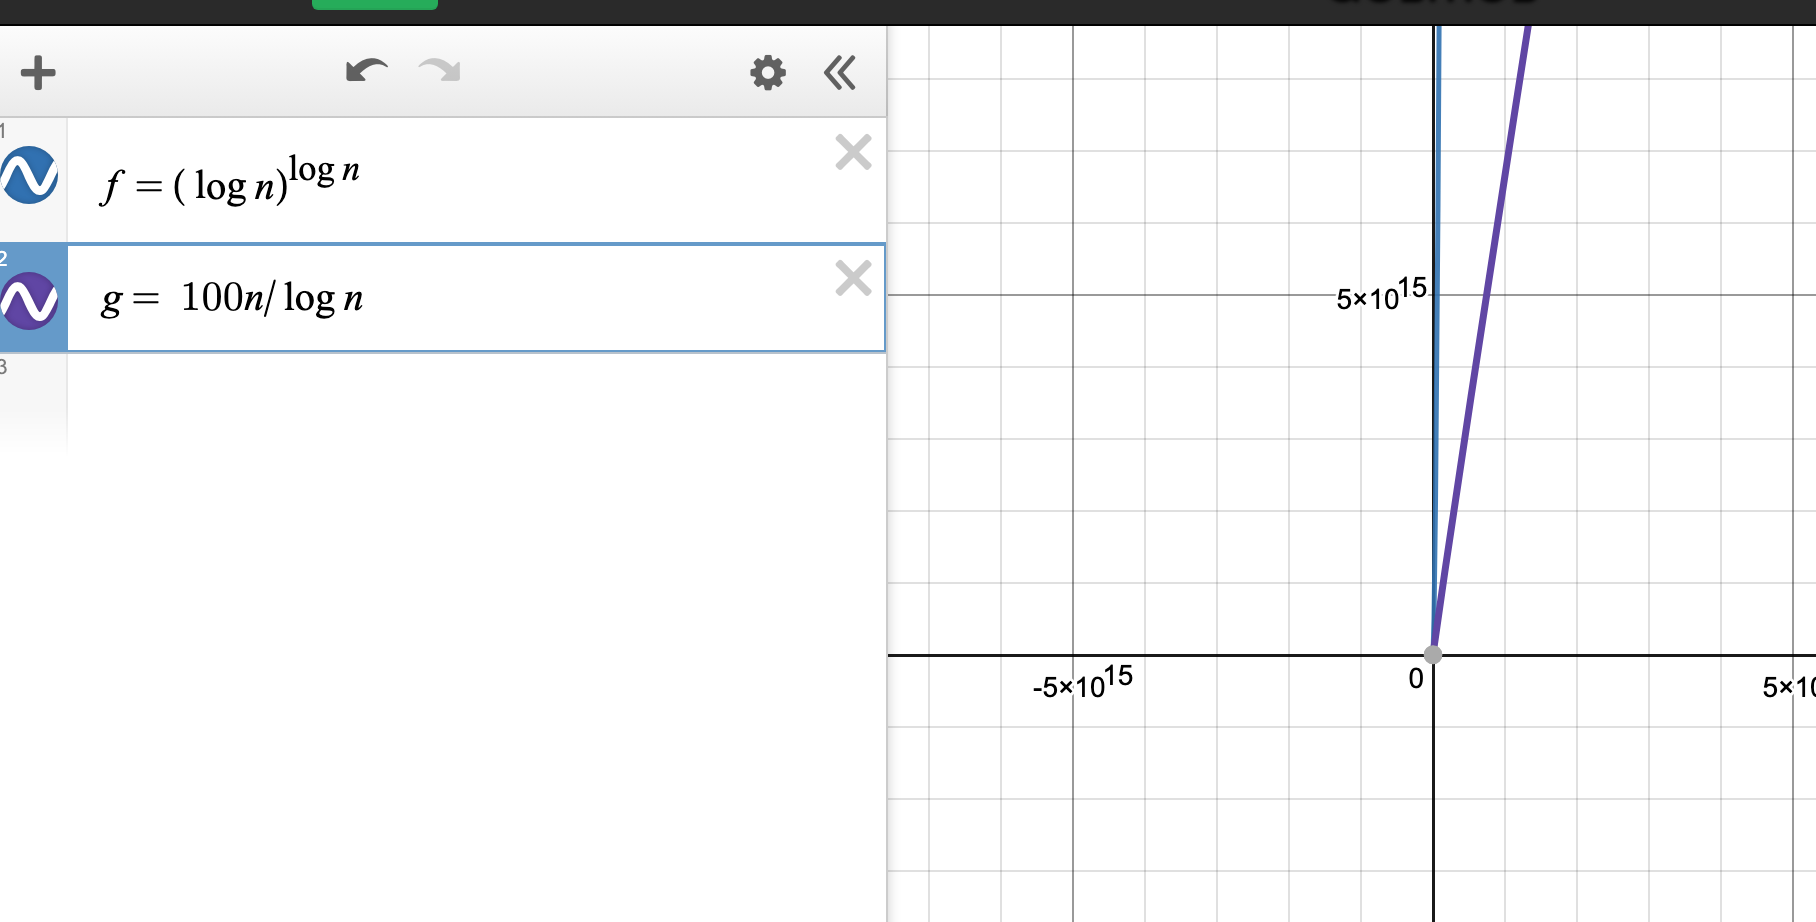
\includegraphics[width=0.9\linewidth, height=4cm]{i) big omega.png}
    \caption{Big Omega}
    \label{fig:subim1}
    \end{subfigure}
    \caption{Image for i)}
    \label{fig:image2}
    \end{figure}
\begin{figure}[h]
\item  this is j
No matter how big C is, C*g(n) can always smaller than f(n) at some point when n $\ge $n0, so there's $f = \Omega(g)$\\
    \begin{subfigure}{0.5\textwidth}
    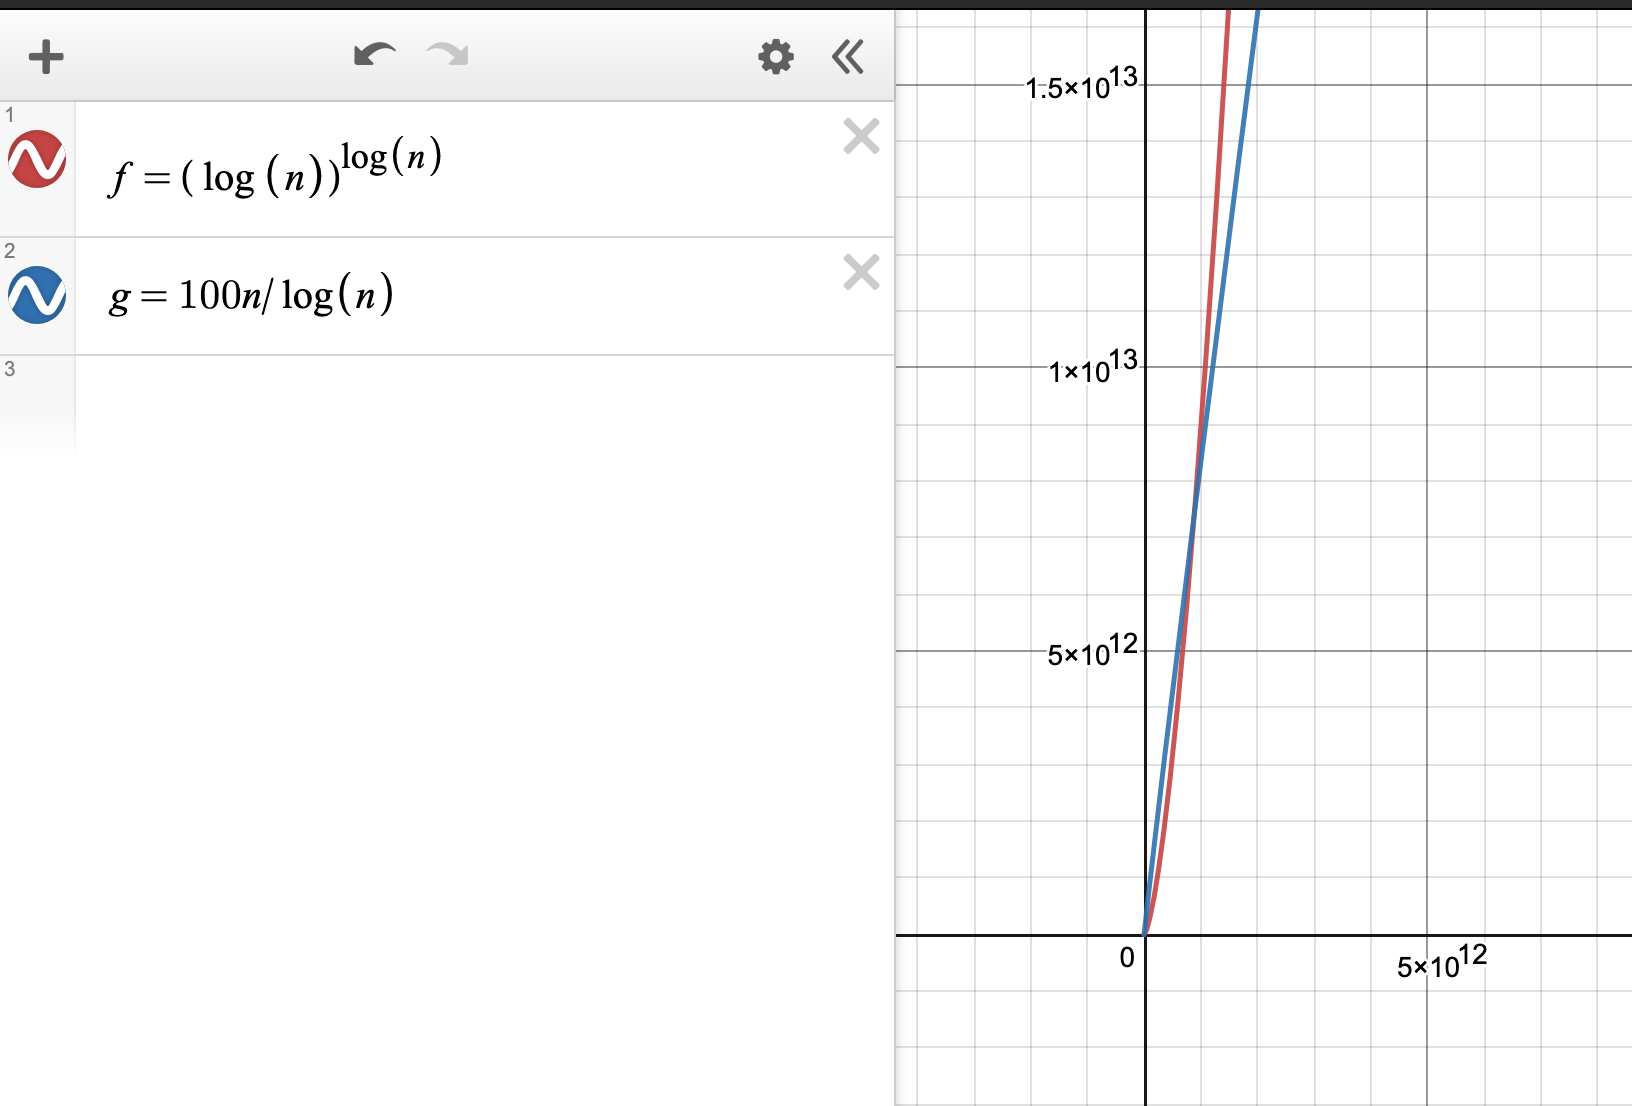
\includegraphics[width=0.9\linewidth, height=4cm]{j) big Omega.png}
    \caption{Big Omega}
    \label{fig:subim1}
    \end{subfigure}
    \caption{Image for i)}
    \label{fig:image2}
    \end{figure} 
\begin{figure}[h]
\item %% this is k
No matter how big C is, C*g(n) can always smaller than f(n) at some point when n $\ge $n0, so there's $f = \Omega(g)$\\
    \begin{subfigure}{0.5\textwidth}
    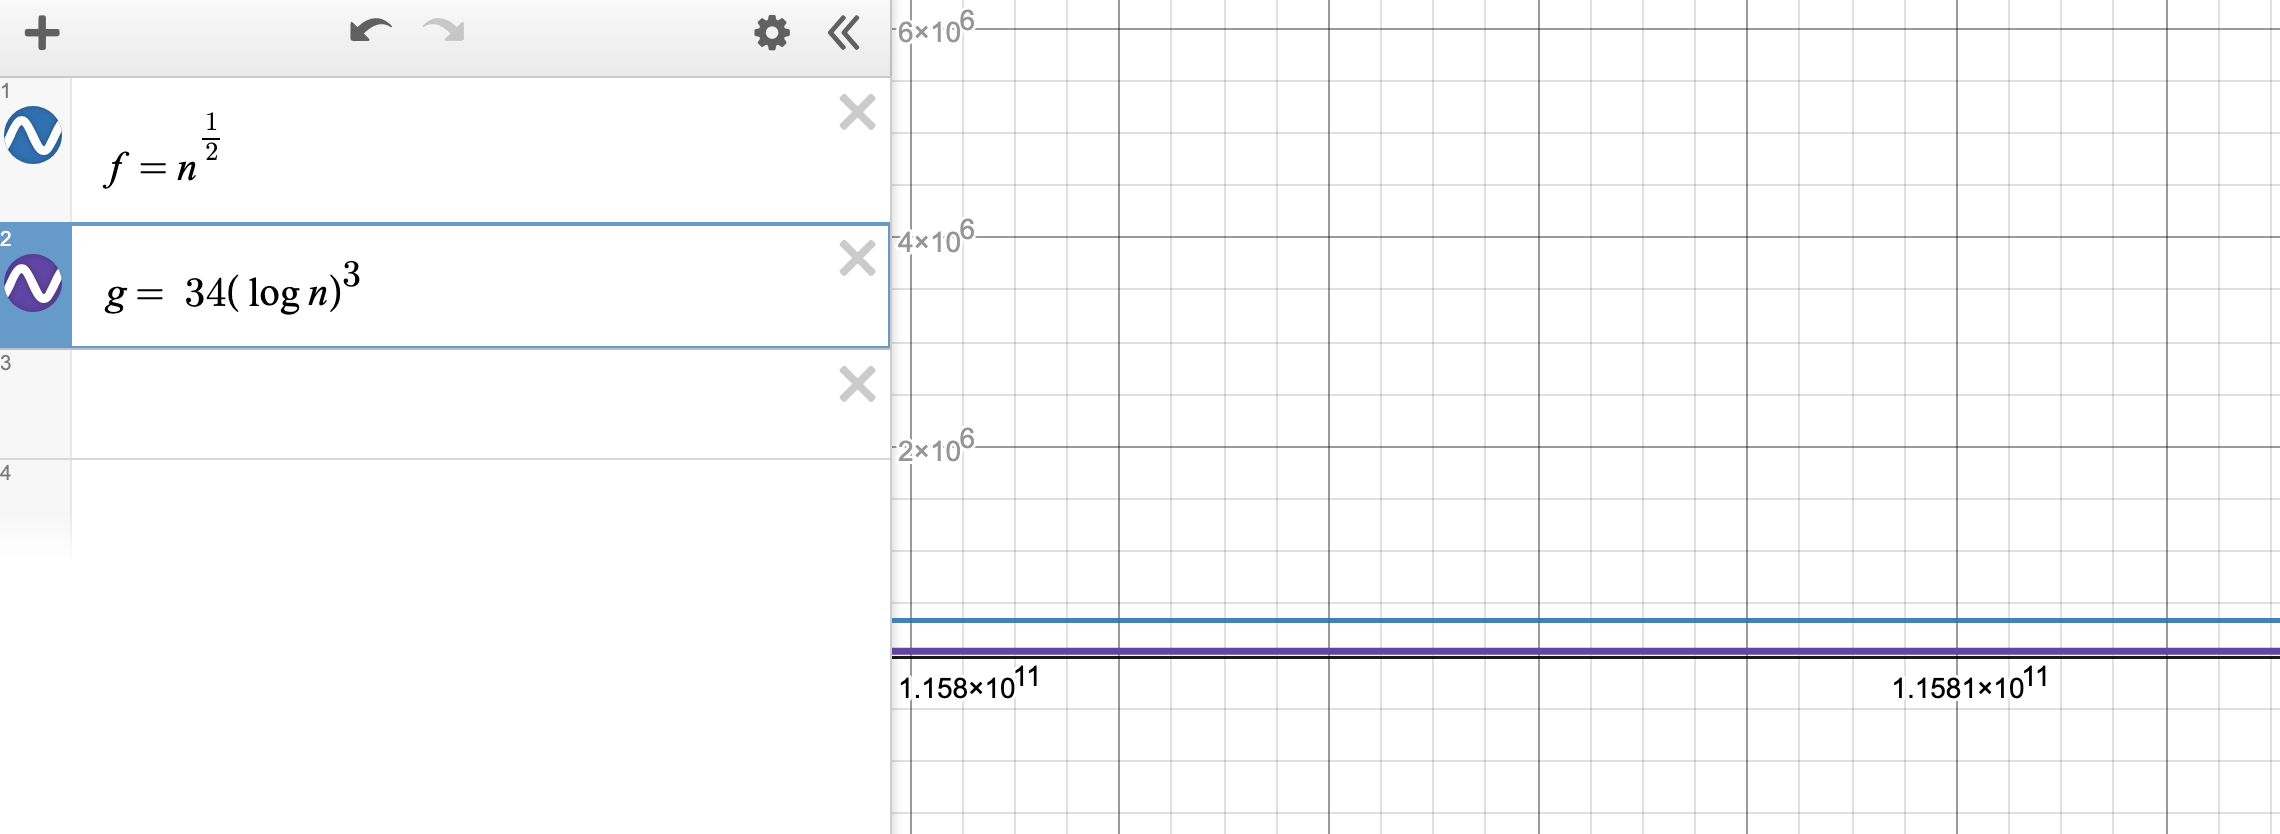
\includegraphics[width=0.9\linewidth, height=4cm]{k) big omega.png}
    \caption{Big Omega}
    \label{fig:subim1}
    \end{subfigure}
    \caption{Image for k)}
    \label{fig:image2}
    \end{figure}

\begin{figure}[h]    
\item %% this is l
No matter how small C is C*g(n) can always bigger than f(n) when n$\ge$n0, so there's f = O(g)\\
    \begin{subfigure}{0.5\textwidth}
    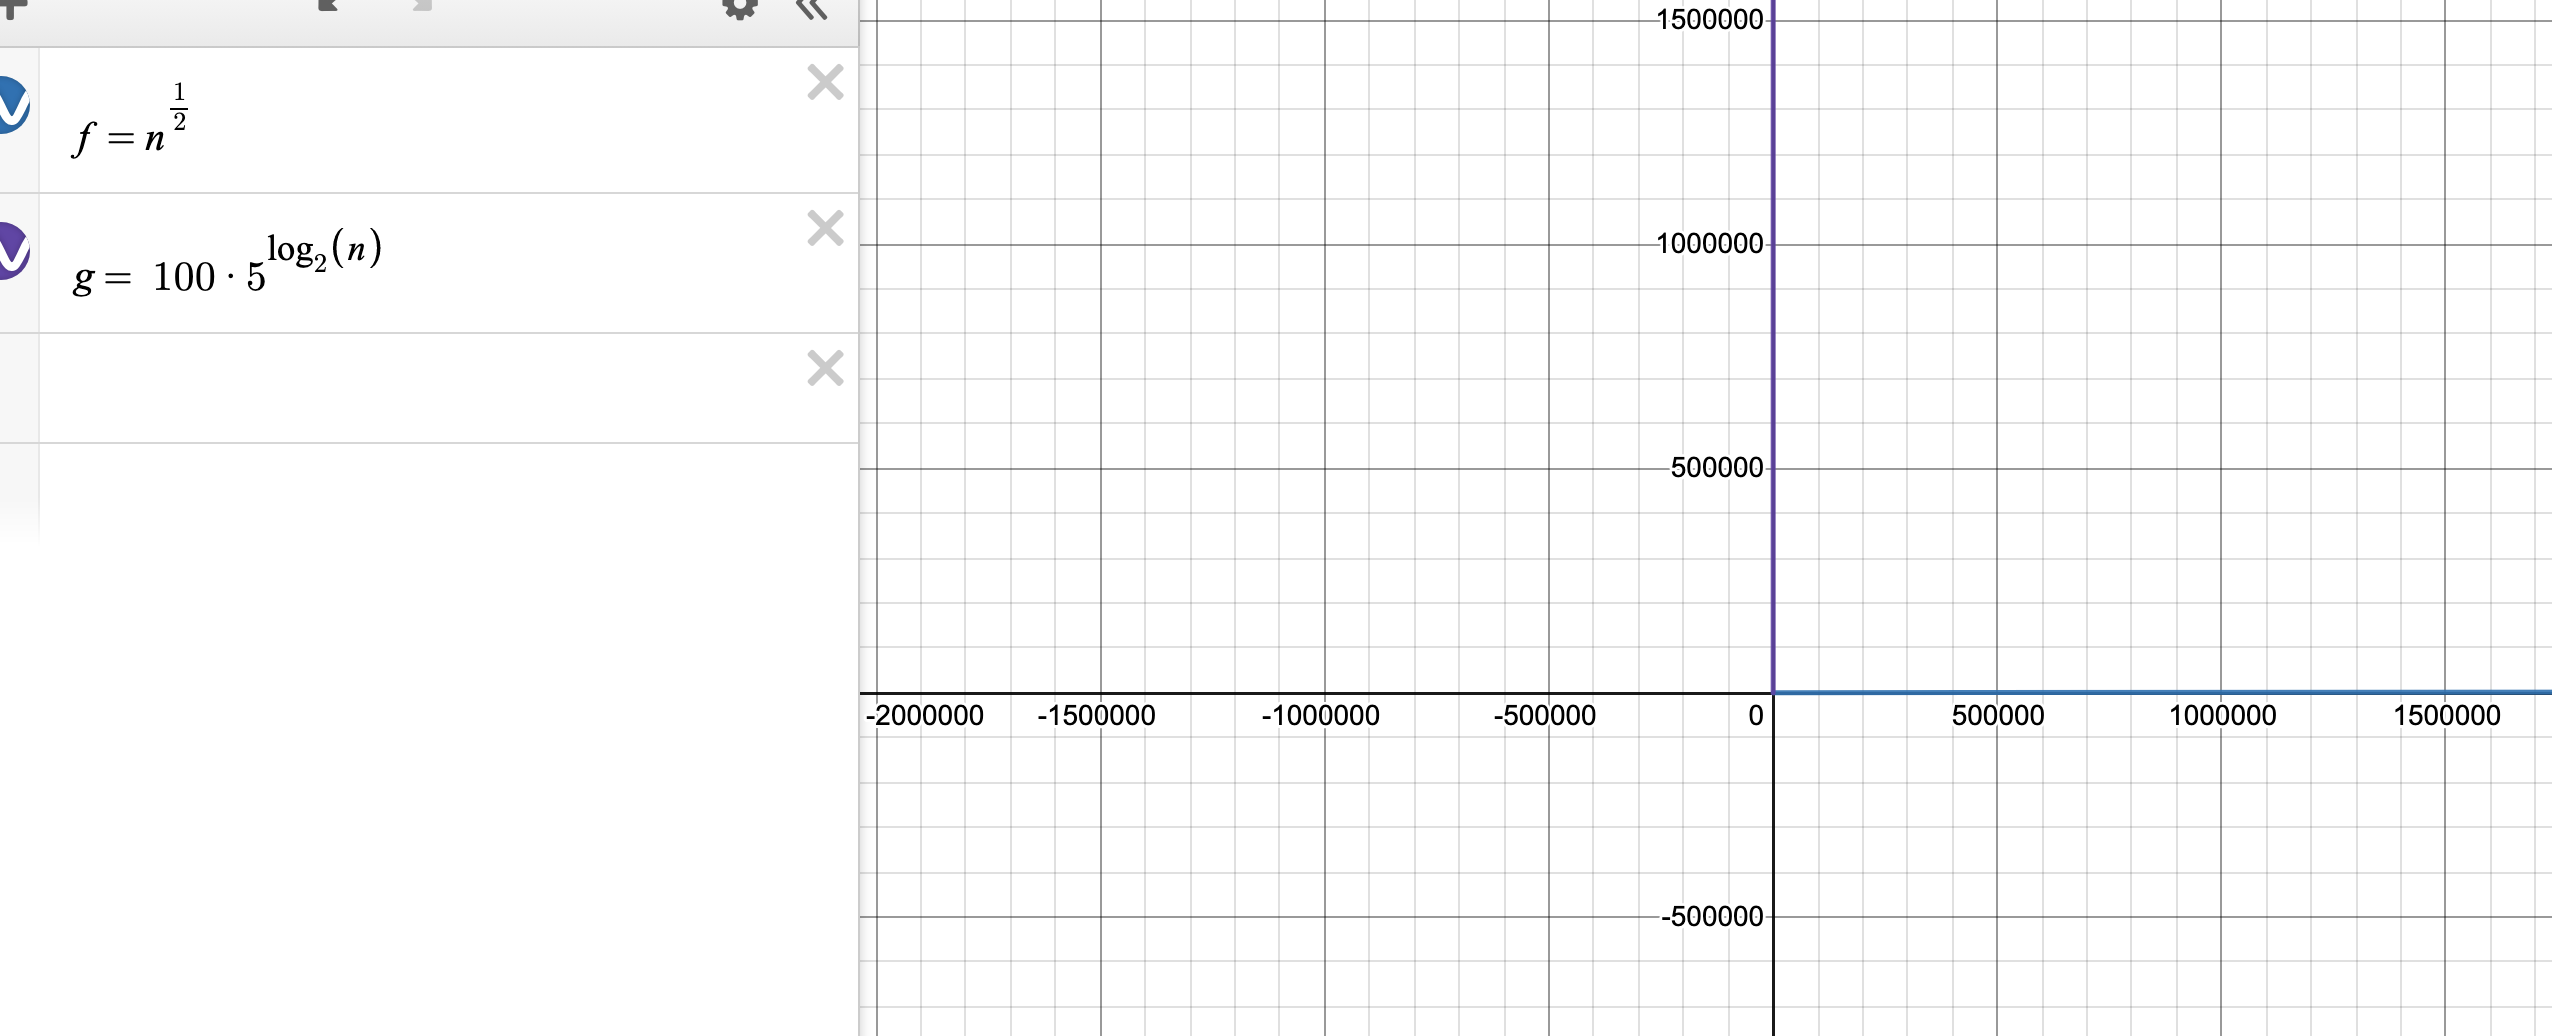
\includegraphics[width=0.9\linewidth, height=4cm]{l) big O.png}
    \caption{Big O}
    \label{fig:subim1}
    \end{subfigure}
    \caption{Image for l)}
    \label{fig:image2}
    \end{figure}

\begin{figure}[h]
\item %% this is m
No matter how small C is C*g(n) can always bigger than f(n) when n$\ge$n0, so there's f = O(g)\\
    \begin{subfigure}{0.5\textwidth}
    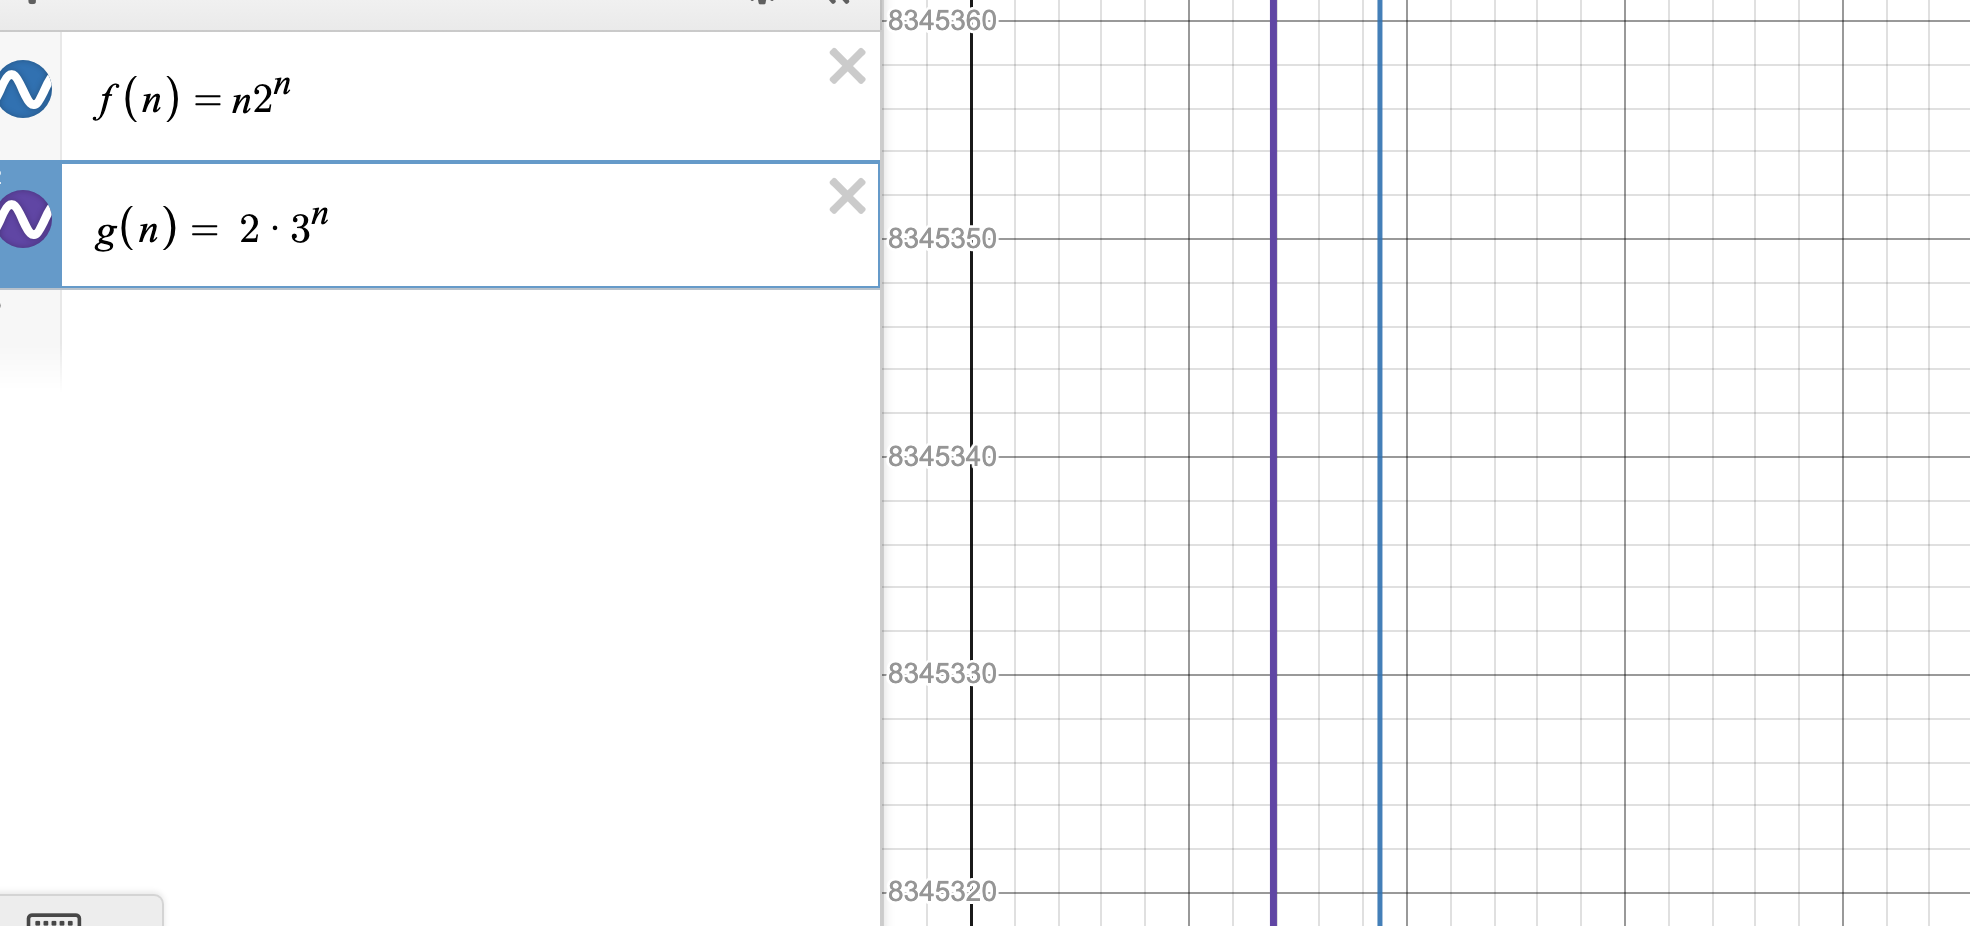
\includegraphics[width=0.9\linewidth, height=4cm]{m big O.png}
    \caption{Big O}
    \label{fig:subim1}
    \end{subfigure}
    \caption{Image for m)}
    \label{fig:image2}
    \end{figure}
 
\begin{figure}[h]  
\item %% this is n
There is C and C' make $C*g(n) \le f(n) \le C'*g(n)$, so  there's f = O(g), f = Omega (g) and f = Theta(g)\\
    \begin{subfigure}{0.5\textwidth}
    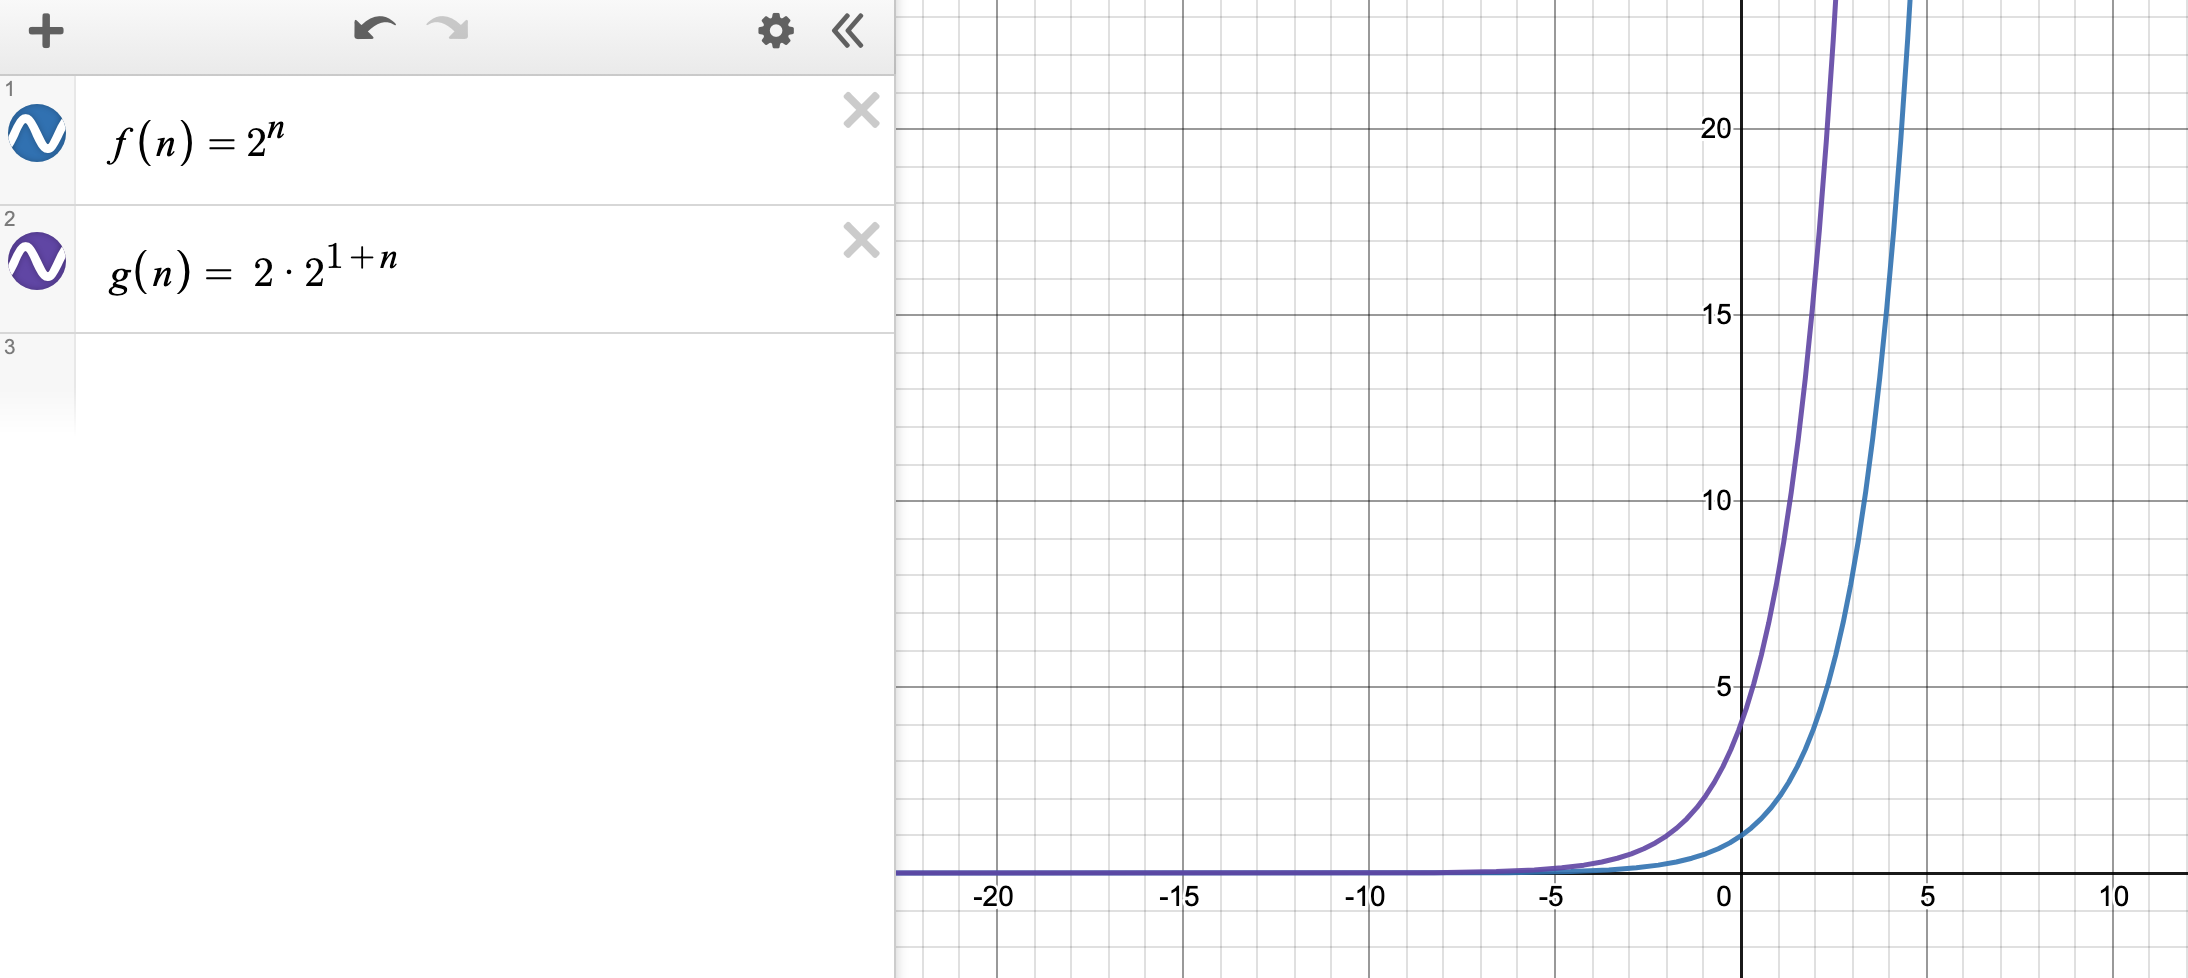
\includegraphics[width=0.9\linewidth, height=4cm]{n big O.png}
    \caption{Big O}
    \label{fig:subim1}
    \end{subfigure}
    \begin{subfigure}{0.5\textwidth}
    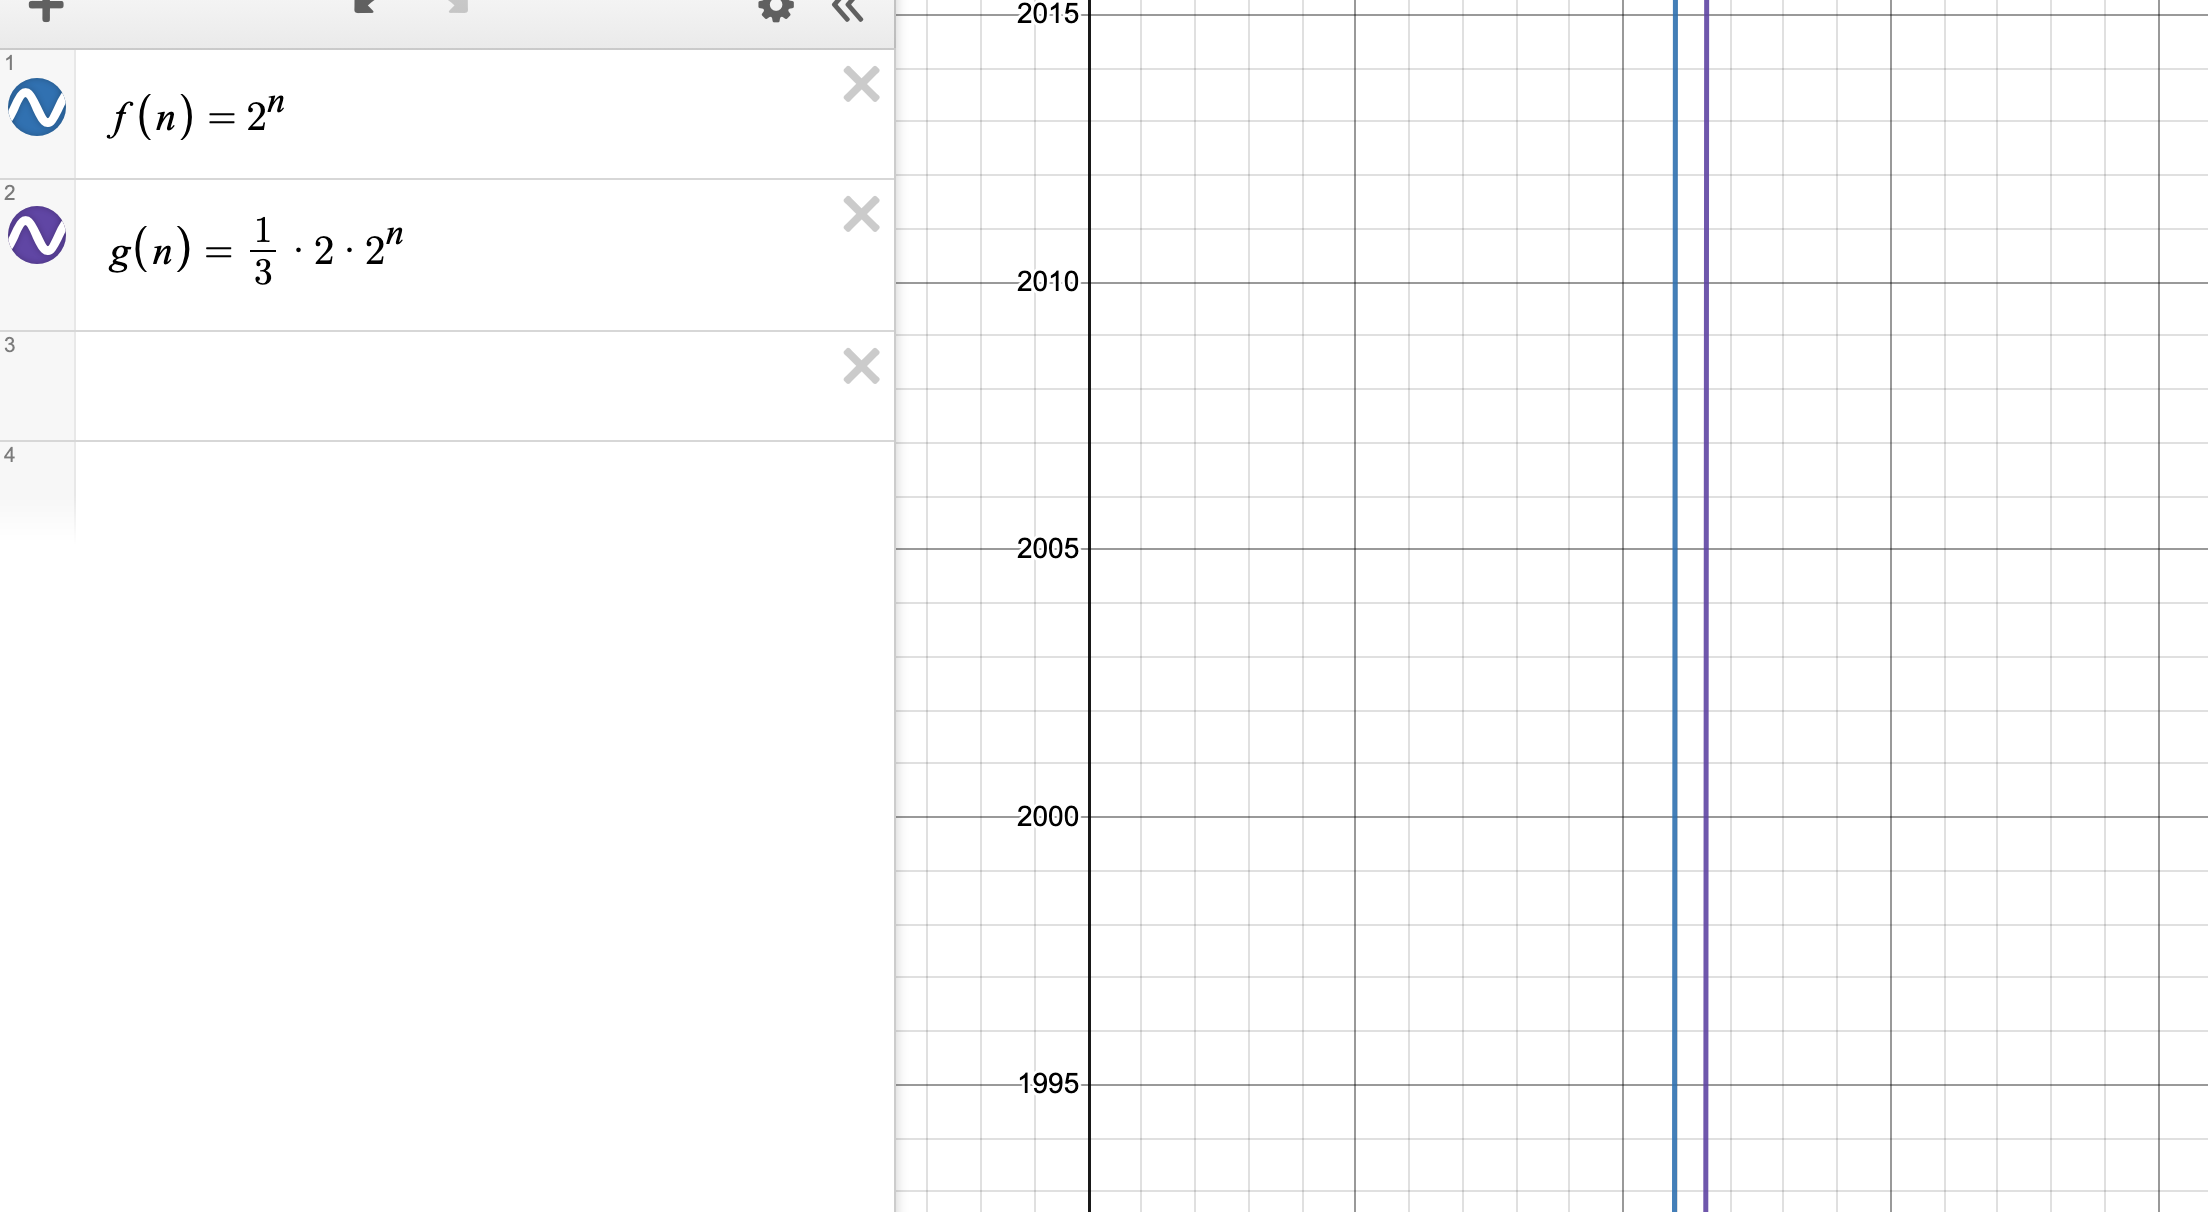
\includegraphics[width=0.9\linewidth, height=4cm]{n big omega.png}
    \caption{Big Omega}
    \label{fig:subim2}
    \end{subfigure}
    \caption{image for n}
    \label{fig:image2}
    \end{figure}
    
\begin{figure}[h]
\item %% this is o
No matter how big C is, C*g(n) can always smaller than f(n) at some point when n $\ge $n0, so there's $f = \Omega(g)$\\
    \begin{subfigure}{0.5\textwidth}
    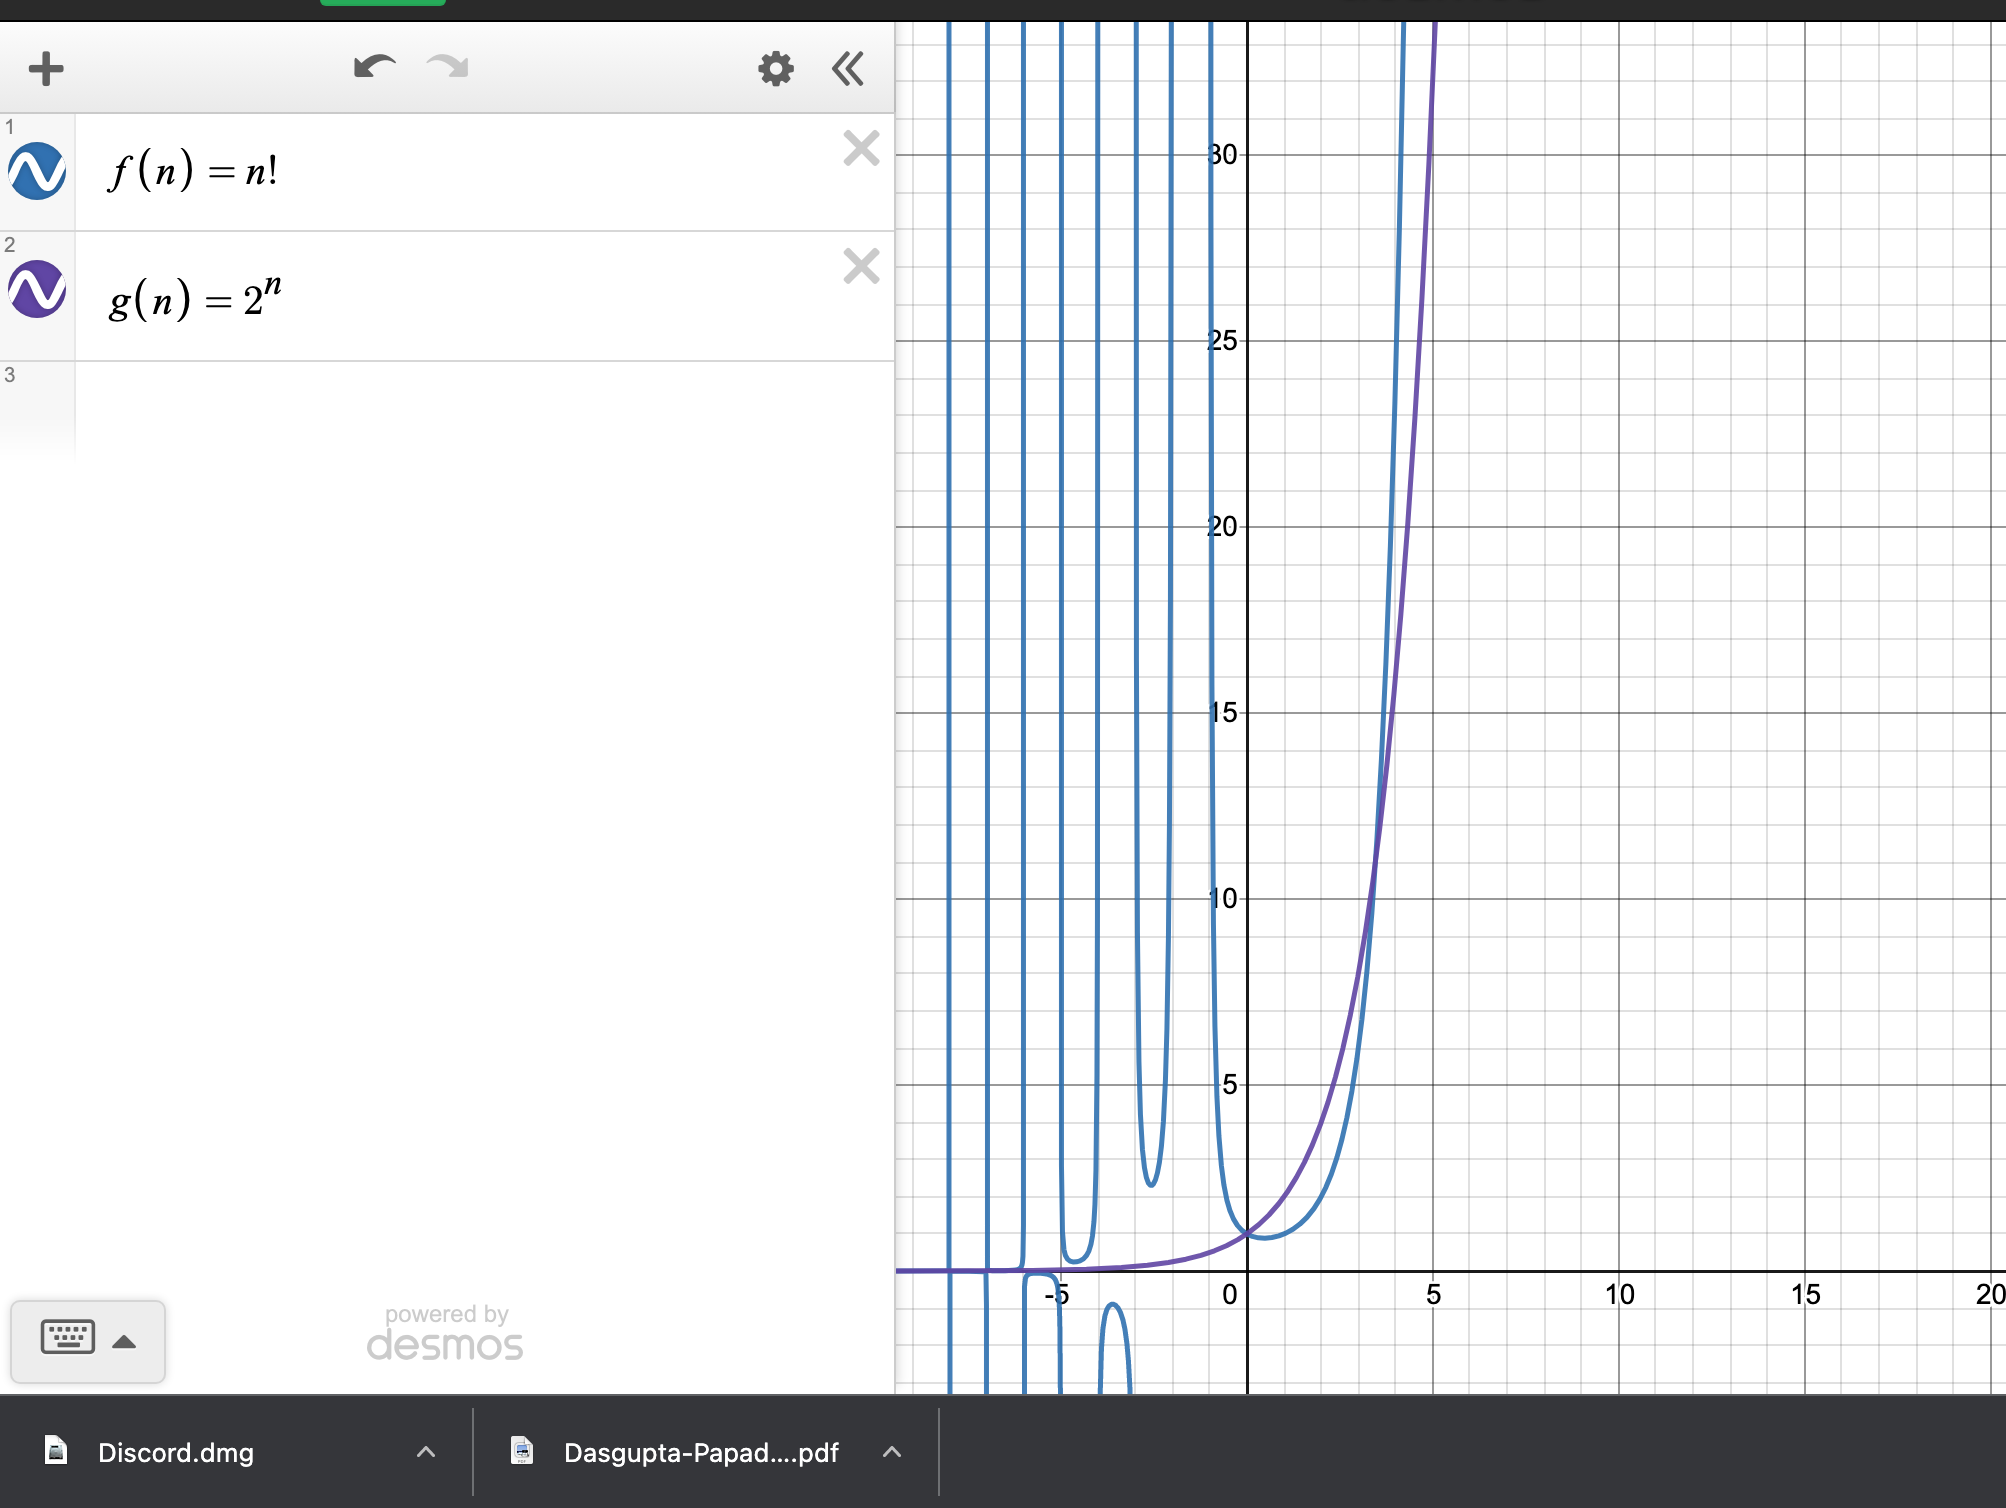
\includegraphics[width=0.9\linewidth, height=4cm]{o big omega.png}
    \caption{Big Omega}
    \label{fig:subim1}
    \end{subfigure}
    \caption{Image for i)}
    \label{fig:image2}
    \end{figure}
    
\begin{figure}[h]
\item %% this is p
No matter how small C is C*g(n) can always bigger than f(n) when n$\ge$n0, so there's f = O(g)\\  
    \begin{subfigure}{0.5\textwidth}
    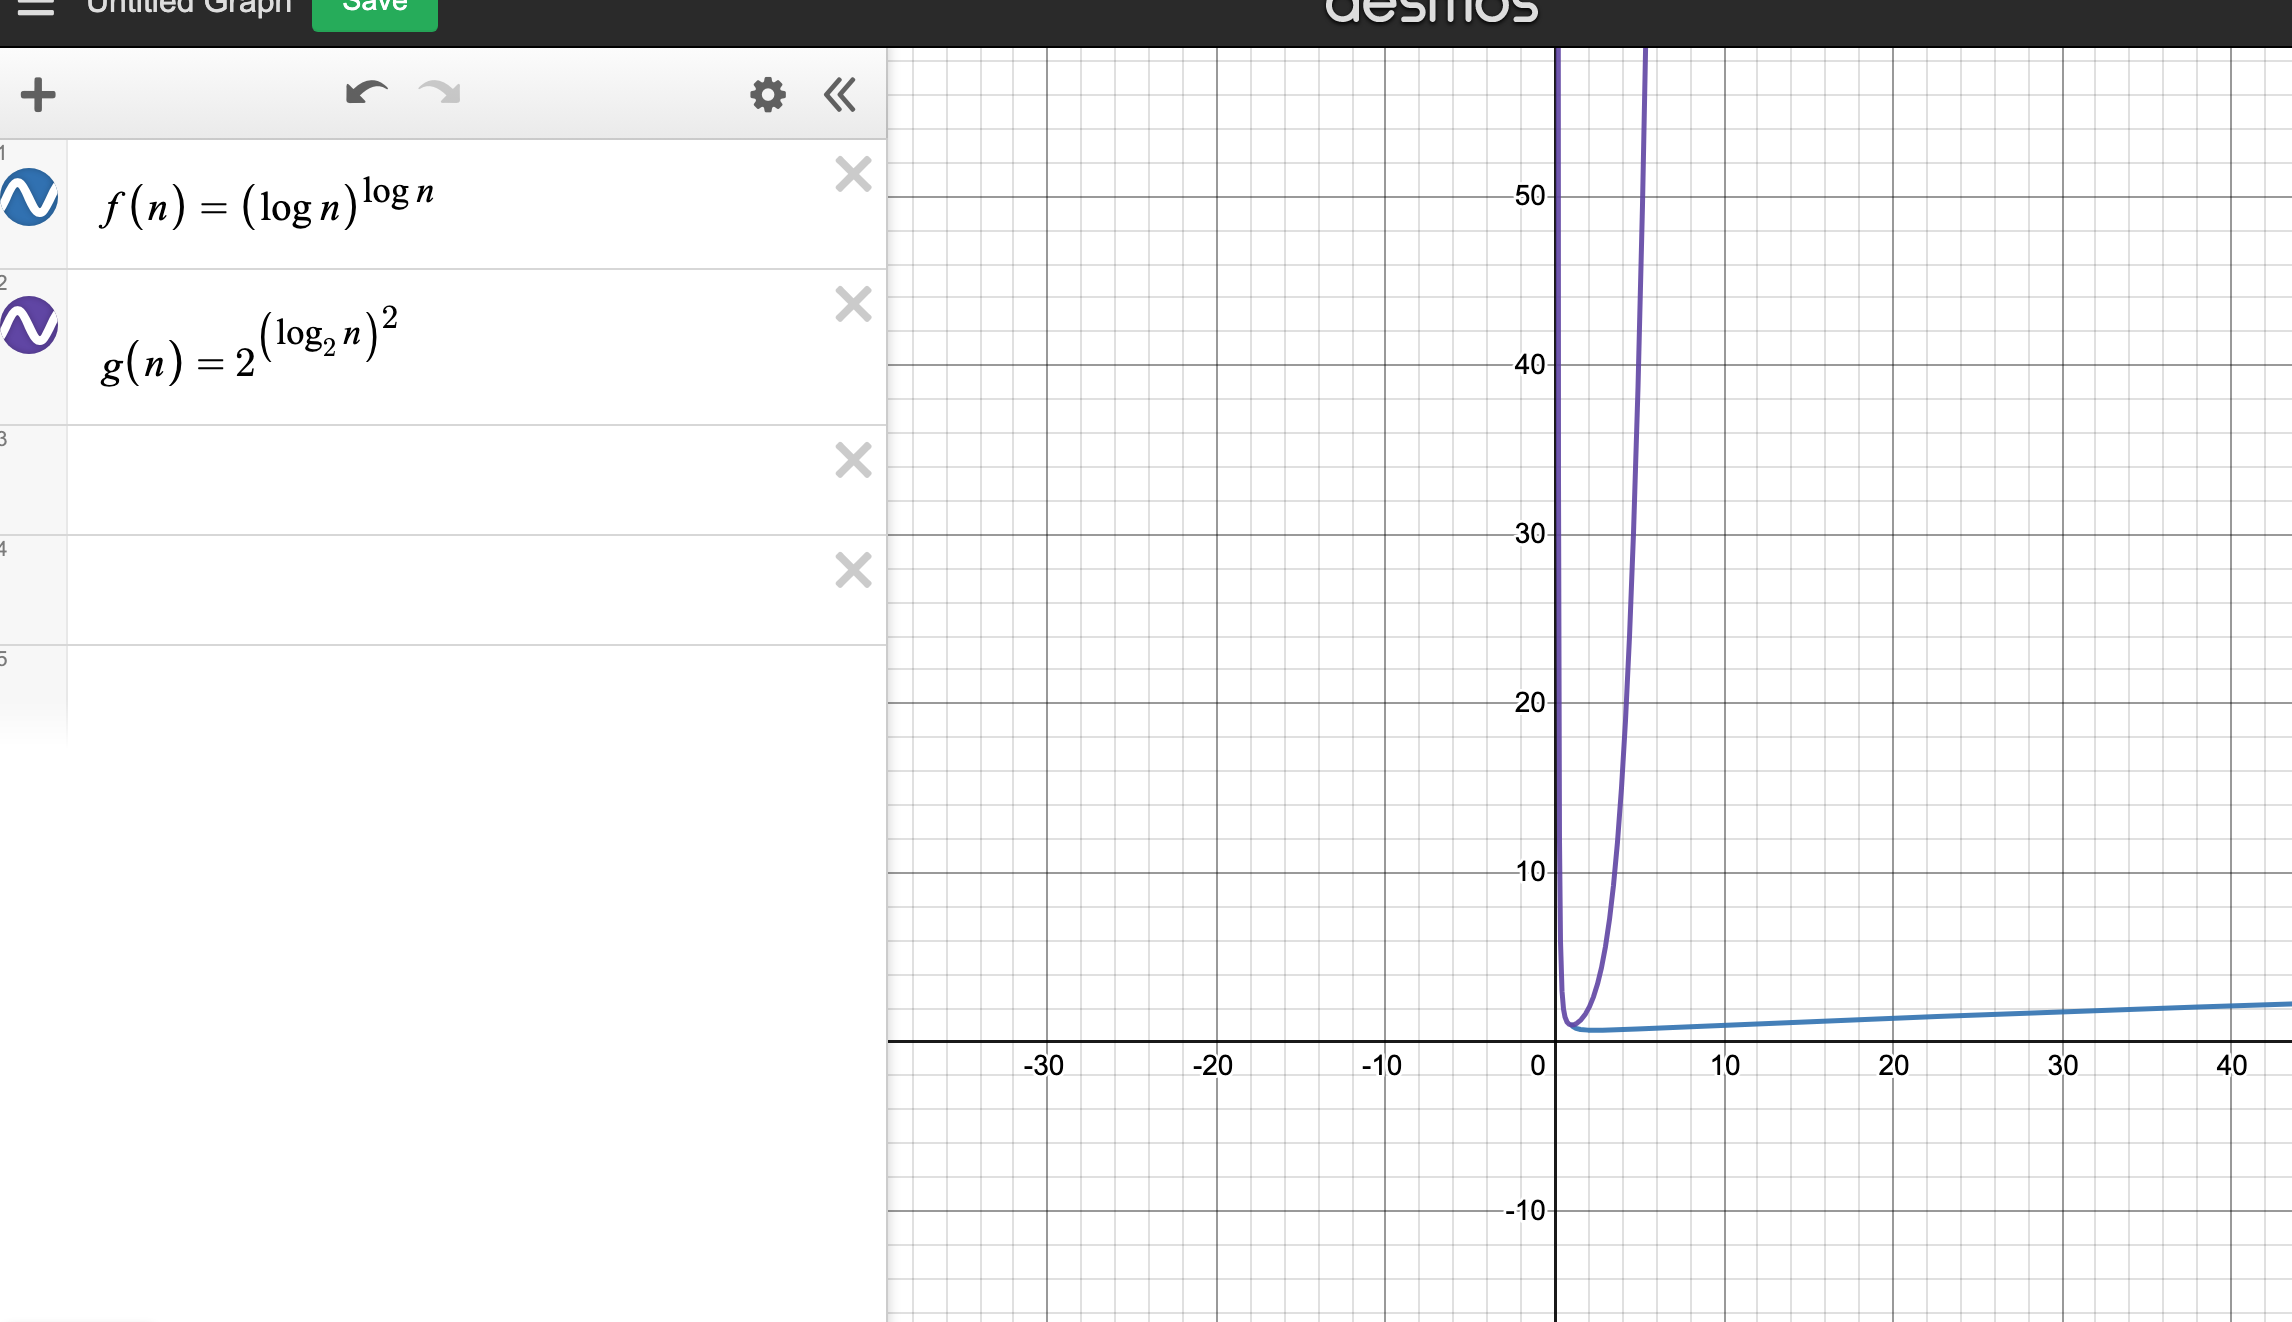
\includegraphics[width=0.9\linewidth, height=4cm]{p big O.png}
    \caption{Big O}
    \label{fig:subim1}
    \end{subfigure}
    \caption{Image for i)}
    \label{fig:image2}
    \end{figure}

\begin{figure}[h]    
\item %% this is q
No matter how big C is, C*g(n) can always smaller than f(n) at some point when n $\ge $n0, so there's $f = \Omega(g)$\\   
    \begin{subfigure}{0.5\textwidth}
    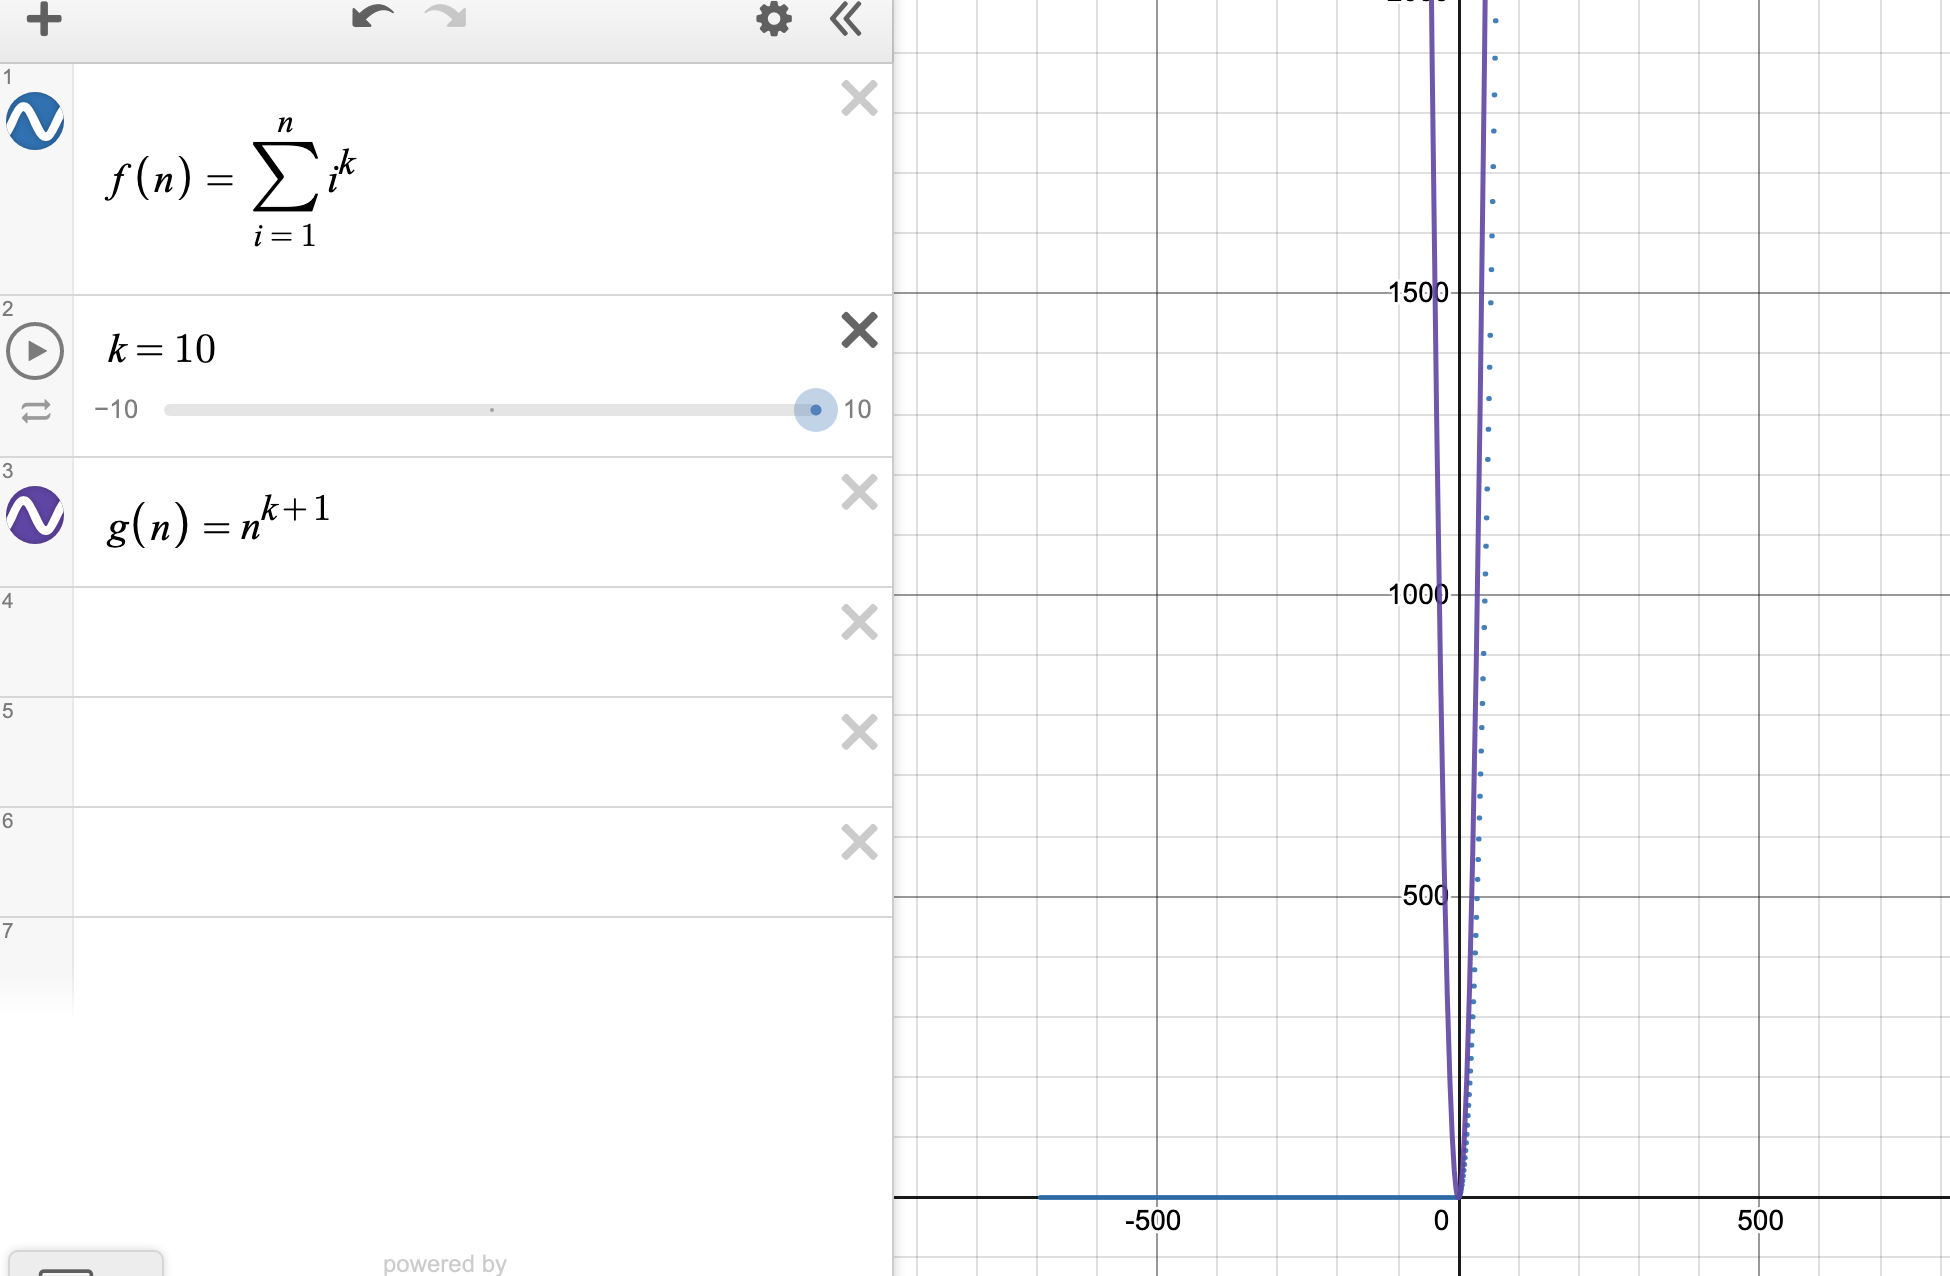
\includegraphics[width=0.9\linewidth, height=4cm]{q big Omega.png}
    \caption{Big Omega}
    \label{fig:subim1}
    \end{subfigure}
    \caption{Image for i)}
    \label{fig:image2}
    \end{figure}
\end{enumerate}


\end{document}
